%%=============================================================================
%% TEMPLATE LATEX -- IDP
%% Instituto Brasileiro de Ensino, Desenvolvimento e Pesquisa
%%
%% Compile com:  latexmk -pdf main.tex
%% (ou:  pdflatex main -> biber main -> pdflatex main -> pdflatex main)
%%
%% Opcoes da classe:
%%   bacharelado | especializacao | mestrado | doutorado  (define a natureza)
%%   secaonovapagina | secaocontinua                      (quebra de capitulo)
%%   semlinks | links                                     (cor dos hiperlinks)
%%   rascunho                                             (marca d'agua)
%%=============================================================================
\documentclass[mestrado]{idp}

%% Pacotes extras que voce quiser usar no seu trabalho ------------------------
\usepackage{amsmath}
\usepackage{array}
\usepackage{longtable}
\usepackage{tikz}
\usetikzlibrary{positioning,arrows.meta,calc,shapes.geometric,fit,backgrounds}

%% Verde institucional usado nos agradecimentos -------------------------------
\definecolor{verdepalmeiras}{HTML}{006437}
%% Latin Modern Typewriter: fonte monoespacada vetorial. A cmtt padrao e
%% bitmap e quebra a expansao automatica do microtype carregado pela classe.
\renewcommand{\ttdefault}{lmtt}
% \usepackage{longtable}
% \usepackage{siunitx}

%% Arquivo de referencias bibliograficas (formato BibTeX) ---------------------
\addbibresource{referencias.bib}

%% Metadados do trabalho ------------------------------------------------------
%%=============================================================================
%% DADOS DO TRABALHO -- FONTE ÚNICA DA VERDADE
%%
%% Este é o ÚNICO arquivo onde os dados do seu trabalho devem ser digitados.
%% Tudo o que aparece na capa, folha de rosto, ficha catalográfica, folha de
%% aprovação e nos metadados do PDF é gerado a partir daqui.
%%
%% Campos marcados como OBRIGATÓRIO que ficarem em branco aparecem no PDF
%% como "[[ PREENCHER: campo ]]" e geram aviso na compilação. Ao gerar a
%% versão final, use a opção `entrega' em main.tex: ela transforma o aviso
%% em erro e impede a compilação com campos pendentes.
%%
%% Para reaproveitar estes dados no corpo do texto, use os acessores:
%%   \TituloTrabalho  \NomeAutor      \NomeOrientador   \NomeCoorientador
%%   \NomeCurso       \NomePrograma   \NomeInstituicao  \AreaConcentracao
%%   \LinhaPesquisa  \LocalTrabalho   \CidadeTrabalho   \AnoTrabalho
%% Exemplo: "Ao meu orientador, \NomeOrientador, agradeço..."
%%=============================================================================

%% --- Identificação ---------------------------------------------------------
%% Título de trabalho, proposto. Ajuste livremente.
\titulo{Exposição ocupacional à inteligência artificial e transições no
        mercado de trabalho brasileiro}                    % OBRIGATÓRIO
\subtitulo{evidências de painel da PNAD Contínua após o lançamento
           público do ChatGPT}                             % opcional
\titulotraduzido{Occupational exposure to artificial intelligence and labor
                 market transitions in Brazil: panel evidence from the
                 Brazilian Continuous National Household Sample Survey after
                 the public release of ChatGPT}             % opcional

\autor{Ricardo Carvalho}                                   % OBRIGATÓRIO
\autorficha{CARVALHO, Ricardo}                             % OBRIGATÓRIO

\orientador{Prof. Dr. Danny de Castro Soares}              % OBRIGATÓRIO
\coorientador{}                                            % opcional

%% --- Vínculo institucional -------------------------------------------------
\curso{}                                 % OBRIGATÓRIO em bacharelado/especialização
\programa{}                              % OBRIGATÓRIO em mestrado/doutorado
\area{}                                  % área de concentração (pós-graduação)
\linhapesquisa{}                         % linha de pesquisa (pós-graduação)

\cidade{Brasília}                        % usada na folha de aprovação
\local{Brasília}                         % usado na capa e folha de rosto
\data{2026}                              % ano de depósito

%% --- Defesa ----------------------------------------------------------------
%% Informe APENAS a data; a cidade vem de \cidade acima.
\datadefesa{}                            % OBRIGATÓRIO -> "Cidade, dd de mes de aaaa."

%% Banca: \membrobanca[Instituição]{Nome}{Função}   (instituição é opcional)
\membrobanca{Prof. Dr. Danny de Castro Soares}{Orientador}
\membrobanca{Prof. Dr. Abel Ferreira}{Examinador interno}
\membrobanca{Prof. Dr. Leonardo Jardim}{Examinador externo}

%% --- Ficha catalográfica ---------------------------------------------------
%% A ficha OFICIAL é elaborada pela Biblioteca Ministro Moreira Alves.
%% Solicite por biblioteca@idp.edu.br e transcreva os dados recebidos aqui.
\cutter{}                                % notação Cutter fornecida pela Biblioteca
\numeropaginas{00}                       % OBRIGATÓRIO: total de folhas
\cdd{XXX}                                % OBRIGATÓRIO: Classificação Decimal de Dewey
\assuntos{}                              % se vazio, usa as palavras-chave

%% --- Resumo ----------------------------------------------------------------
\palavraschave{Inteligência artificial. Mercado de trabalho. Mobilidade
               ocupacional. Informalidade. PNAD Contínua.}  % OBRIGATÓRIO
\keywords{Artificial intelligence. Labor market. Occupational mobility.
          Informality. Brazilian household survey.}         % OBRIGATÓRIO


\begin{document}

%%=============================== PRE-TEXTUAL ================================
\pretextual

\capa                    % Capa (obrigatorio, nao e contada na paginacao)
\folhaderosto            % Folha de rosto (obrigatorio, folha 1)
\fichacatalografica      % Ficha catalografica (obrigatorio)
\folhadeaprovacao        % Folha de aprovacao (obrigatorio)

%% DEDICATORIA (elemento opcional)
%% Texto breve, no final da página, alinhado a 8 cm da margem esquerda.
%% Nao leva titulo.

\begin{dedicatoria}
% NOTA DE TRABALHO: escrita por último, junto com a introdução e o resumo.
[[ A escrever ao final. ]]
\end{dedicatoria}
      % opcional
%% AGRADECIMENTOS (elemento opcional)
%% Texto de gratificacao a pessoas e/ou instituicoes que contribuiram de
%% maneira relevante para o desenvolvimento do trabalho ou para a conclusao
%% do curso.

\begin{agradecimentos}
Agradeço, em primeiro lugar, a Deus, pela vida, pela saúde, pela força e por me
permitir chegar até aqui. Pela sabedoria nos momentos de decisão, pela
serenidade nos momentos difíceis e pelas pessoas que colocou em meu caminho ao
longo desta jornada. Em cada desafio, encontrei forças para continuar e, em
cada conquista, motivos para agradecer. Chegar ao fim desta etapa é também
reconhecer que nenhuma caminhada é feita apenas por nossas próprias forças.

Agradeço ao meu orientador, \NomeOrientador, pelo rigor, pela paciência e,
principalmente, por insistir que método vem antes de resultado. Mais do que
orientar esta pesquisa, Danny foi um exemplo de professor que sabe cuidar de
seus alunos. É impossível não perceber o brilho em seus olhos quando compartilha
conhecimento e a dedicação com que transforma dúvidas e dificuldades em
aprendizado. Nunca imaginei que um doido pelo Flamengo aceitaria colocar um
doido pelo Palmeiras como seu orientando e, mais do que isso, dedicaria tanto do
seu tempo, conhecimento, paciência e carinho para que pudéssemos chegar juntos
até aqui. Professor, muito obrigado por acreditar neste trabalho e, sobretudo,
por mostrar que uma boa orientação vai muito além das páginas de uma
dissertação.

Agradeço aos professores Prof. Dr. Abel Ferreira e Prof. Dr. Leonardo Jardim,
que aceitaram compor a banca e dedicar seu tempo e conhecimento à leitura e
avaliação deste trabalho. Agradeço também a todos os professores e servidores do
Instituto Brasileiro de Ensino, Desenvolvimento e Pesquisa (IDP), pela formação
recebida, pelas discussões, pelos ensinamentos e pelo apoio ao longo dessa
caminhada acadêmica.

À CAIXA ECONÔMICA FEDERAL, instituição da qual tenho enorme orgulho de fazer
parte, registro meu profundo agradecimento pela oportunidade e pelo investimento
em minha formação, especialmente pela concessão da bolsa que possibilitou a
realização deste mestrado. Agradeço aos meus gestores, Dario de Paula e Rodrigo
Batista, que foram grandes incentivadores desta jornada, compreenderam a
importância desse projeto e me estimularam a seguir em frente. De maneira muito
especial, agradeço à minha parceira de equipe na GEFET02, Patrícia, que
inúmeras vezes ``segurou a barra'' enquanto eu precisava me ausentar para
estudar, assistir às aulas ou cumprir as atividades do mestrado. Nenhuma
formação acontece de maneira verdadeiramente individual, e ter pessoas que
acreditam, incentivam e ajudam a criar as condições para que possamos estudar
faz toda a diferença.

À minha turma do mestrado, carinhosamente apelidada de GIT, meu muito obrigado.
Foram aulas, trabalhos, discussões, apresentações, mensagens, dúvidas, risadas e
muitos momentos compartilhados que tornaram essa caminhada muito mais leve. Em
especial, agradeço aos meus parceiros Mairton e Kelsen e à mulher mais sinistra
da turma, Fabiana. Cada um, do seu jeito, fez parte desta história. O mestrado
me entregou conhecimento e um título, mas também me deu pessoas que quero levar
comigo muito além da sala de aula.

À minha família, minha base e minha maior conquista, faltariam páginas para
agradecer tudo o que representam em minha vida. À minha esposa, Lucilene, minha
companheira de caminhada, obrigado pelo amor, pela paciência, pelo apoio e por
compreender todas as vezes em que o mestrado ocupou um tempo que deveria ser
nosso. Seu incentivo nos dias de cansaço e sua presença constante nos momentos
de dúvida tornaram esta caminhada possível, e esta conquista é tão sua quanto
minha. Aos meus filhos, Daniela e André Ricardo, vocês são uma das principais
razões pelas quais procuro evoluir todos os dias. Ver vocês crescerem é o maior
orgulho que carrego, e foi pensando em vocês que encontrei ânimo para seguir nos
momentos mais difíceis. Espero que, ao olharem para esta conquista, entendam que
estudar, aprender e buscar novos desafios não têm idade e que nossos sonhos
exigem dedicação. Se este trabalho lhes ensinar alguma coisa, que seja isto:
nunca parem de aprender.

Aos meus irmãos, José Bento, Rosa, Sônia, Eliene e Célia, e aos meus cunhados e
cunhadas, agradeço pelo carinho, pela torcida e por toda uma vida compartilhada
em família. Cada um, à sua maneira, faz parte da história que me trouxe até aqui
e das lembranças, aprendizados e momentos que ajudaram a formar quem sou. E aos
meus amados pais, Antônio e Edite, meu agradecimento mais profundo. Vocês sempre
nos mostraram, muito mais por atitudes do que por palavras, a importância da
família para a vida. Ensinaram que podemos estudar, trabalhar, conquistar
posições e alcançar nossos objetivos, mas que nenhuma dessas conquistas terá o
mesmo significado se não tivermos pessoas para amar e com quem compartilhá-las.
Muito do homem, do pai e do profissional que sou nasceu dos valores que aprendi
dentro de casa com vocês. Esta conquista também é de vocês.

Aos grandes amigos que a vida colocou no meu caminho, meu irmão de vida
Geovane, Brunno, Luiz Abul, Jonenson, Malafaia, Leila, Carolzinha, Lucas,
Marcão, Manu, Liana, Cléber, Tinho, Ygor e Leandro, deixo meu agradecimento
especial. Vocês estiveram presentes de diferentes formas, incentivando,
torcendo, ouvindo, aconselhando e, muitas vezes, simplesmente lembrando que
existe vida além de artigo, banco de dados, regressão e dissertação. Amizade de
verdade também é entender a ausência sem transformar a distância em
afastamento. Obrigado por acreditarem em mim, por vibrarem com minhas conquistas
e, principalmente, por fazerem parte da minha vida nos momentos importantes.

Faço também um agradecimento que carrega saudade. Ao meu padrinho Sebastião da
Cunha, que nos deixou em agosto de 2026. Sebastião foi muito mais que meu
cunhado e padrinho: foi, para mim, como um pai. Entre tantas coisas que me
ensinou, talvez as maiores tenham sido aquelas que não estão nos livros: ser uma
pessoa boa, estar disponível para ajudar os outros, cuidar das pessoas e, acima
de tudo, saber viver feliz. Sua forma simples, prestativa e alegre de encarar a
vida deixou marcas que o tempo não apagará. Gostaria muito que estivesse aqui
para compartilhar este momento, mas sei que muito do que aprendi com você
continuará comigo por toda a vida. Obrigado, padrinho. Esta conquista também
leva um pouco de você.

E, para fechar estes agradecimentos, não poderia deixar de falar de uma paixão
que me acompanha por toda a vida: o \textcolor{verdepalmeiras}{Palmeiras}. O
\textcolor{verdepalmeiras}{Palmeiras} me ensinou algo que nenhuma regressão é
capaz de ensinar: campanha longa se ganha com
\textcolor{verdepalmeiras}{constância}, resultado ruim em um trimestre não
decide a temporada e \textcolor{verdepalmeiras}{disciplina} tática é o que
sustenta o talento nos dias em que a inspiração não aparece. Foi com a mesma
\textcolor{verdepalmeiras}{paciência} de quem acompanha um campeonato inteiro
que este trabalho foi construído, rodada a rodada, trimestre a trimestre,
corrigindo a estratégia quando necessário, respeitando o processo e entendendo
que nenhuma partida isolada define o campeonato.

Talvez seja justamente essa uma das maiores lições desta caminhada. Na pesquisa,
assim como no futebol e na vida, nem sempre a primeira tentativa dá certo. Há
resultado que decepciona, modelo que precisa ser refeito, hipótese que não se
confirma e momentos em que parece que o objetivo está distante. Mas quem
acredita no processo continua trabalhando. Esta dissertação foi construída
assim, com constância, disciplina e a certeza de que o campeonato só termina no
apito final.

A todos que estiveram comigo nesta caminhada, de perto ou de longe, meu muito
obrigado. Esta dissertação leva meu nome na capa, mas carrega, em suas páginas,
um pouco de cada pessoa que me ajudou a chegar até aqui.

Avanti, Palestra!

% Escudo oficial de 1942: Wikimedia Commons, File:Palmeiras_logo.svg (PD-textlogo;
% marca registrada da Sociedade Esportiva Palmeiras).
\begin{center}
  
\includegraphics[height=2cm]{figuras/palmeiras.png}
\end{center}
\end{agradecimentos}
   % opcional
%% EPIGRAFE (elemento opcional)
%% Citacao seguida da indicacao de autoria, relacionada ao tema do trabalho.
%% Nao leva titulo.

\begin{epigrafe}
``Cabeça fria, coração quente.''
\end{epigrafe}
         % opcional
%% RESUMO NA LINGUA VERNACULA (elemento obrigatorio -- NBR 6028)
%% Paragrafo unico, 150 a 500 palavras: objetivo, metodo, resultados, conclusao.
%% Termina com as palavras-chave (ja vem de \palavraschave em config/dados.tex).

\begin{resumo}
% NOTA DE TRABALHO: o resumo é escrito por último, junto com a introdução e as
% considerações finais, quando os resultados estiverem estabilizados. A estrutura
% da NBR 6028 é: objetivo, método, resultados e conclusão, em parágrafo único de
% 150 a 500 palavras, sem citações e sem enumeração de tópicos.
[[ A escrever ao final, junto com a introdução. ]]
\end{resumo}
           % obrigatorio
%% RESUMO EM LINGUA ESTRANGEIRA (elemento obrigatorio -- NBR 6028)
%% Versao fiel do resumo.tex, na lingua estrangeira escolhida (geralmente ingles).

\begin{abstract}
% WORKING NOTE: written last, as a faithful translation of resumo.tex.
[[ To be written at the end, mirroring resumo.tex. ]]
\end{abstract}
         % obrigatorio

\listailustracoes        % opcional -- alimentada por \caption em figure
\listatabelas            % opcional -- alimentada por \caption em table
\listaquadros            % opcional -- alimentada por \caption em quadro
\listagraficos           % opcional -- alimentada por \caption em grafico

%% LISTA DE ABREVIATURAS E SIGLAS (elemento opcional)
%% Ordem alfabetica. Use \sigla{SIGLA}{significado por extenso}.

\begin{siglas}
  \sigla{ABNT}{Associação Brasileira de Normas Técnicas}
  \sigla{AIOE}{\textit{Artificial Intelligence Occupational Exposure} --- índice de exposição ocupacional à inteligência artificial}
  \sigla{CNAE}{Classificação Nacional de Atividades Econômicas}
  \sigla{CNPJ}{Cadastro Nacional da Pessoa Jurídica}
  \sigla{COD}{Classificação de Ocupações para Pesquisas Domiciliares}
  \sigla{DD}{Diferenças em diferenças}
  \sigla{DP}{Desvio-padrão}
  \sigla{IA}{Inteligência artificial}
  \sigla{IBGE}{Instituto Brasileiro de Geografia e Estatística}
  \sigla{IDP}{Instituto Brasileiro de Ensino, Desenvolvimento e Pesquisa}
  \sigla{IPW}{\textit{Inverse probability weighting} --- ponderação pelo inverso da probabilidade de resposta}
  \sigla{ISCO}{\textit{International Standard Classification of Occupations}}
  \sigla{LLM}{\textit{Large language model} --- modelo de linguagem de grande porte}
  \sigla{MPL}{Modelo de probabilidade linear}
  \sigla{p.p.}{Pontos percentuais}
  \sigla{PNADC}{Pesquisa Nacional por Amostra de Domicílios Contínua}
  \sigla{SOC}{\textit{Standard Occupational Classification}}
  \sigla{UF}{Unidade da Federação}
  \sigla{UPA}{Unidade Primária de Amostragem}
\end{siglas}
           % opcional

\sumario                 % obrigatorio

%%================================= TEXTUAL ==================================
\textual

\section{Introdução}

%%=============================================================================
%% NOTA DE TRABALHO -- LEIA ANTES DE ESCREVER
%%
%% A INTRODUÇÃO É A ÚLTIMA COISA QUE ESCREVEREMOS.
%%
%% Motivo: a introdução tem de prometer exatamente o que o trabalho entrega.
%% Enquanto a especificação, a amostra e a leitura dos resultados ainda estão
%% se estabilizando (Capítulos 3 e 4), qualquer introdução escrita agora vira
%% dívida: promete efeito causal onde há associação condicional, promete
%% horizonte longo onde a margem é trimestral, promete "impacto da IA" onde o
%% tratamento é um índice ocupacional. Escrevemos a introdução, o resumo e o
%% abstract juntos, no fim, a partir do que os Capítulos 3, 4 e 5 já disserem.
%%
%% Ordem de escrita combinada: Capítulo 3 -> Capítulo 4 -> Capítulo 5 ->
%% Capítulo 2 (fechamento da literatura) -> Capítulo 1 -> resumo/abstract.
%%=============================================================================

Esta seção será redigida ao final, depois de fechados os procedimentos
metodológicos, os resultados preliminares e as considerações. O objetivo é
garantir que a promessa feita aqui corresponda exatamente ao que o desenho
identifica e ao que os dados sustentam.

Quando for escrita, a introdução deverá cobrir, nesta ordem:

\begin{enumerate}[label=\alph*)]
  \item \textbf{contextualização}: a difusão de modelos de linguagem de grande
        porte a partir do lançamento público do ChatGPT, em 30 de novembro de
        2022, e por que esse marco é usado como referência temporal;
  \item \textbf{problema de pesquisa}: trabalhadores em ocupações mais expostas
        à inteligência artificial passaram a apresentar transições de trabalho
        diferentes (mudança de ocupação, saída do emprego, informalização,
        deslocamento no gradiente de exposição) depois desse marco?
  \item \textbf{hipóteses}: as hipóteses de trabalho que serão confrontadas com
        os desfechos do Capítulo~\ref{sec:resultados}, escritas de forma que
        possam ser rejeitadas;
  \item \textbf{objetivo geral e objetivos específicos}: medir o gradiente
        condicional de transição ocupacional por desvio-padrão de exposição e
        descrever a mobilidade entre faixas de exposição, deixando explícito que
        a validação do desenho (estudo de evento, testes de tendência
        pré-marco e bateria de sensibilidade) fica para a agenda do
        Capítulo~\ref{sec:melhorias};
  \item \textbf{justificativa}: a inexistência, no Brasil, de medida direta de
        adoção de inteligência artificial em bases representativas, e o que uma
        medida de exposição ocupacional aplicada a um painel domiciliar
        rotativo permite e não permite concluir;
  \item \textbf{delimitação}: o que o trabalho \emph{não} pretende identificar,
        antecipando a Seção~\ref{sec:limites};
  \item \textbf{estrutura do texto}: um parágrafo apresentando os cinco
        capítulos.
\end{enumerate}

% TODO: substituir todo o conteúdo acima pelo texto final da introdução.

\section{Revisão de literatura}

Este capítulo é construído em duas camadas. A primeira, apresentada na
Seção~\ref{sec:leituras}, é uma proposta de leitura: cinco artigos que
sustentam, em conjunto, as principais escolhas relativas à medida de exposição
e à estratégia de identificação adotadas no Capítulo~\ref{sec:metodo}; decisões
como pareamento, ponderação e inferência têm justificativa própria naquele
capítulo. Não são cinco textos escolhidos por proximidade
temática genérica com o tema ``inteligência artificial e trabalho'', e sim os
cinco textos de que este trabalho depende para justificar, respectivamente, a
medida de tratamento, a medida alternativa de exposição, o que se sabe sobre o
efeito de produtividade da ferramenta, o que se sabe sobre o efeito agregado no
mercado de trabalho e o desenho de identificação por exposição diferencial. A
segunda camada, nas seções seguintes, é a revisão propriamente dita, construída a partir dessas leituras e ampliada com a literatura brasileira de
mobilidade ocupacional e informalidade.

\subsection{Proposta de leitura}
\label{sec:leituras}

O Quadro~\ref{qua:leituras} lista as cinco leituras propostas, na ordem em que
convém lê-las. A ordem não é cronológica: começa pela medida que este trabalho
usa como tratamento, passa pela medida concorrente, desce ao nível da firma e
do trabalhador e termina no desenho econométrico que serve de modelo ao
Capítulo~\ref{sec:metodo}.

\begin{quadro}[htb]
  \caption{Proposta de leitura, na ordem sugerida}
  \label{qua:leituras}
  \centering
  \espacosimples\idpcorpodez
  \begin{tabular}{@{}p{0.5cm}p{4.3cm}p{9.4cm}@{}}
    \toprule
    \textbf{\#} & \textbf{Referência} & \textbf{Por que ler} \\
    \midrule
    1 & \citeonline{felten2021}
      & Define o AIOE, que é literalmente a variável de tratamento deste
        trabalho. Sem esse texto não se sabe o que o coeficiente mede. \\
    \addlinespace
    2 & \citeonline{eloundou2024}
      & Medida concorrente de exposição, específica a modelos de linguagem.
        É a primeira robustez prevista no Capítulo~\ref{sec:melhorias}. \\
    \addlinespace
    3 & \citeonline{brynjolfsson2025}
      & Efeito estimado com adoção observada e implantação escalonada. Serve de
        contraste: mostra o que este trabalho não consegue observar. \\
    \addlinespace
    4 & \citeonline{humlum2025}
      & Desenho com exposição ocupacional e horizonte curto, com efeitos nulos
        e precisos. Referência para calibrar a expectativa de magnitude. \\
    \addlinespace
    5 & \citeonline{acemoglu2020}
      & Modelo canônico de identificação por exposição diferencial e leitura
        de deslocamento \emph{versus} recomposição. \\
    \bottomrule
  \end{tabular}
  \fonte{Elaboração própria (2026).}
\end{quadro}

As subseções a seguir retomam essas leituras na ordem do
Quadro~\ref{qua:leituras}, e todas seguem o mesmo percurso: sintetizam,
inicialmente, a contribuição do artigo e, na sequência, explicitam por que a
leitura importa para esta dissertação, seja pela decisão de desenho que
sustenta, seja pelo limite que ajuda a reconhecer. A coluna ``Por que ler'' do
quadro antecipa, em forma resumida, o argumento que cada subseção desenvolve.
Lidas em conjunto, as cinco leituras formam a base sobre a qual se apoiam as
seções seguintes deste capítulo e as escolhas metodológicas apresentadas no
Capítulo~\ref{sec:metodo}.

\subsubsection{Felten, Raj e Seamans (2021)}

\citeonline{felten2021} constroem o \textit{Artificial Intelligence
Occupational Exposure} (AIOE), índice que liga aplicações correntes de
inteligência artificial às habilidades exigidas por cada ocupação e, a partir
daí, produz um escore de exposição por ocupação da classificação ocupacional
americana. O índice é padronizado entre ocupações, de modo que uma unidade
corresponde aproximadamente a um desvio-padrão de exposição.

Trata-se do artigo mais importante da lista por uma razão simples: o AIOE é o
tratamento deste trabalho, e sua leitura responde às dúvidas que o leitor tende
a formular diante do índice. O AIOE mede a exposição potencial de cada ocupação
às aplicações de inteligência artificial, e não a adoção efetivamente observada
da tecnologia, seus efeitos sobre a produtividade ou o risco de substituição do
trabalho. A padronização entre ocupações, por sua vez, define a escala em que se
leem os coeficientes estimados no Capítulo~\ref{sec:resultados}, expressos por unidade do índice. Por fim, exposição elevada não deve ser tomada como
sinônimo de ocupação pior, pois o índice descreve a proximidade entre as
habilidades requeridas pela ocupação e as capacidades da tecnologia, e não a
qualidade do emprego. Essa distinção precisa estar clara antes de qualquer
interpretação distributiva dos resultados.

\subsubsection{Eloundou et al. (2024)}

\citeonline{eloundou2024} propõem uma medida de exposição construída
especificamente para modelos de linguagem de grande porte, avaliando tarefa a
tarefa se o acesso a um modelo reduziria substancialmente o tempo de execução.
Estimam que cerca de 80\% da força de trabalho americana teria ao menos 10\%
das tarefas afetadas e que aproximadamente 19\% teria ao menos metade delas.

A leitura é necessária por uma razão de robustez. O AIOE foi construído antes
da difusão dos modelos generativos e capta exposição à inteligência artificial
em sentido amplo; a medida de \citeonline{eloundou2024} é contemporânea ao
choque que este trabalho usa como marco temporal. Se as duas medidas produzem
gradientes de sinal e magnitude semelhantes, o resultado é mais crível; se
divergem, a divergência informa qual dimensão de exposição está de fato
correlacionada com as transições observadas. A substituição da medida de
exposição está registrada como primeira melhoria posterior na
Seção~\ref{sec:exposicoes}.

\subsubsection{Brynjolfsson, Li e Raymond (2025)}

\citeonline{brynjolfsson2025} acompanham a implantação escalonada de um
assistente conversacional em uma central de atendimento e medem ganho de
produtividade, com efeitos concentrados entre trabalhadores menos experientes.
A estratégia apoia-se na observação da adoção, na variação do momento de
implantação entre equipes e na medição do desfecho no nível do trabalhador;
como em todo desenho de implantação escalonada, a leitura causal depende de que
esse momento não esteja associado a tendências próprias das equipes.

O artigo entra na lista como contraste metodológico deliberado. Ele mostra o
que se consegue afirmar quando a adoção é observada e o que, por consequência,
não se consegue afirmar quando ela não é. Neste trabalho não há adoção
observada: há um índice ocupacional e um marco temporal nacional. A comparação com \citeonline{brynjolfsson2025} delimita, assim, o que os
coeficientes do Capítulo~\ref{sec:resultados} podem e não podem sustentar.

\subsubsection{Humlum e Vestergaard (2025)}

\citeonline{humlum2025} combinam levantamentos representativos de adoção de
assistentes conversacionais com registros administrativos vinculados de
empregador e empregado na Dinamarca. Estimam efeitos nulos e precisos sobre
rendimentos e horas, descartando efeitos superiores a poucos pontos percentuais
dois anos após a adoção, e encontram recomposição de tarefas e alguma troca de
ocupação sem variação líquida de horas ou remuneração. O texto circulou
inicialmente com o título \textit{Large Language Models, Small Labor Market
Effects}.

É o artigo cuja leitura mais muda a expectativa sobre a magnitude dos
resultados. O desenho compartilha elementos com o deste trabalho (diferenças em
diferenças, exposição ocupacional e horizonte curto), mas usa dados
administrativos muito mais ricos e examina desfechos e populações distintos. O
achado central, de que a margem que se move é a de composição de tarefas e de
troca de ocupação, e não a de emprego ou salário, é parcialmente compatível com
o padrão dos resultados do Capítulo~\ref{sec:resultados}, em que o coeficiente
estatisticamente mais forte é o de deslocamento no gradiente de exposição, e não
o de saída do emprego. Trata-se de compatibilidade parcial, e não de
confirmação, dadas as diferenças de desenho, população e desfecho.

\subsubsection{Acemoglu e Restrepo (2020)}

\citeonline{acemoglu2020} estimam o efeito da adoção de robôs industriais sobre
emprego e salários em mercados de trabalho locais americanos, usando a exposição
diferencial desses mercados à robotização. É o desenho canônico de identificação
por exposição diferencial e a referência padrão para a distinção entre efeito de
deslocamento e efeito de recomposição.

A leitura serve a dois propósitos. O primeiro é metodológico: o trabalho mostra
como se argumenta a favor de uma medida de exposição como fonte de variação
identificadora e, mais importante, quais objeções essa estratégia atrai:
tendências pré-existentes, choques setoriais concomitantes, seleção na medida de
exposição. Todas reaparecem no Capítulo~\ref{sec:metodo}. O segundo é conceitual:
a decomposição entre deslocamento e recomposição dá vocabulário para interpretar
por que a permanência ocupacional cai em todas as faixas de exposição no período
analisado, e não apenas nas mais expostas.

\subsection{Inteligência artificial, automação e mercado de trabalho}

A literatura econômica sobre automação e trabalho organiza-se em torno de uma
decomposição que \citeonline{acemoglu2019} formalizaram no quadro de tarefas.
Toda tecnologia que passa a executar tarefas antes desempenhadas por pessoas
produz, ao mesmo tempo, um \emph{efeito de deslocamento}, que reduz a demanda
por trabalho nas tarefas automatizadas, e um \emph{efeito de recomposição}, que
a amplia nas tarefas remanescentes, nas novas tarefas criadas pela própria
tecnologia e nos setores beneficiados pelo ganho de produtividade. O sinal do
efeito líquido não é, por isso, uma predição teórica: é uma questão empírica,
cuja resposta depende de qual dos dois efeitos domina em cada horizonte e em
cada mercado. A onda anterior de automação (robótica industrial e
informatização de rotinas) alcançou sobretudo tarefas codificáveis e
repetitivas, concentradas em ocupações de escolaridade intermediária, e a
evidência de \citeonline{acemoglu2020} para mercados de trabalho locais
americanos, construída sobre a exposição diferencial desses mercados à
robotização, indica predomínio do deslocamento nesse caso. Dessa literatura este
trabalho herda não apenas o vocabulário, mas a estratégia de identificação: usar
a exposição diferencial à tecnologia como fonte de variação, com as objeções que
ela atrai e que reaparecem no Capítulo~\ref{sec:metodo}.

A inteligência artificial generativa desloca essa fronteira. Diferentemente da
automação de rotinas, ela alcança tarefas cognitivas não rotineiras (redigir,
resumir, programar, atender), historicamente protegidas por exigirem
linguagem e julgamento, e concentradas em ocupações de escolaridade alta. A
predição de viés de rotina, que orientou a leitura distributiva da onda
anterior, deixa de valer automaticamente: não há razão \textit{a priori} para
que a exposição à inteligência artificial se distribua na mesma direção da
exposição à robotização, e é justamente por isso que a direção do gradiente
precisa ser estimada em vez de suposta. A evidência disponível até aqui, porém,
é mais contida do que o debate público sugere, e convém não tomá-la como bloco
homogêneo, porque os dois trabalhos de referência medem objetos distintos.
\citeonline{brynjolfsson2025} documentam ganhos de produtividade concentrados
entre trabalhadores menos experientes, em desenho com adoção observada no
interior de uma única firma: é evidência sobre desempenho individual na execução
da tarefa, não sobre emprego ou salário agregados. \citeonline{humlum2025}, com
registros administrativos vinculados e adoção declarada em escala nacional,
estimam efeitos nulos e precisos sobre rendimentos e horas dois anos após a
adoção, e observam recomposição de tarefas e alguma troca de ocupação: é
evidência sobre resultados agregados de mercado, não sobre produtividade
individual. As duas são complementares, e não redundantes: a primeira mostra
que a ferramenta entrega ganho onde é adotada; a segunda, que esse ganho ainda
não se converteu em deslocamento mensurável de renda ou de horas no horizonte
observado. Tomadas em conjunto, tornam plausível que a margem de ajuste mais
provável no curto prazo seja a de composição e realocação, e é essa expectativa,
e não a de destruição líquida de postos, que orienta a leitura dos
resultados no Capítulo~\ref{sec:resultados}.

\subsection{Medidas de exposição ocupacional à inteligência artificial}

As medidas de exposição ocupacional à inteligência artificial usadas na
literatura empírica dividem-se em duas famílias, e a diferença entre elas não é
de calibragem, mas de objeto. A primeira parte das \emph{habilidades}
requeridas pelas ocupações: o AIOE de \citeonline{felten2021} associa aplicações
de inteligência artificial às habilidades requeridas pelas ocupações e agrega
essa correspondência em um escore padronizado entre ocupações. Mede, portanto,
quanto do repertório de habilidades de uma ocupação está ao alcance da
tecnologia. A segunda parte das \emph{tarefas}: \citeonline{eloundou2024}
avaliam, atividade a atividade, se o acesso a um modelo de linguagem reduziria
em pelo menos metade o tempo necessário para executá-la, mantendo a qualidade do
resultado, e agregam esse veredito em uma fração de tarefas expostas. Mede,
portanto, quanto do que a ocupação faz poderia ser feito mais rapidamente com o
auxílio da ferramenta. As duas recorrem à mesma fonte ocupacional americana
(o O*NET), mas a dimensões distintas dela: o AIOE parte do inventário de
habilidades associadas a cada ocupação, ao passo que a medida de
\citeonline{eloundou2024} parte das atividades de trabalho detalhadas e das
tarefas. Respondem, por isso, a perguntas diferentes, e nada garante que ordenem
as ocupações da mesma maneira.

A escolha entre elas condiciona a interpretação dos coeficientes. O AIOE é
anterior à difusão dos modelos generativos e capta exposição à inteligência
artificial em sentido amplo, o que o torna adequado a um desenho cujo marco
temporal é o lançamento público de uma ferramenta específica apenas sob a
hipótese de que a ordenação das ocupações por exposição ampla se aproxima da
ordenação por exposição generativa; a medida de \citeonline{eloundou2024} é
contemporânea ao choque e dispensa essa hipótese, mas é específica a modelos de
linguagem e, por construção, desconsidera aplicações de inteligência artificial
que não passem por texto. Este trabalho adota o AIOE como tratamento e registra
a substituição pela medida alternativa como primeira robustez prevista na
Seção~\ref{sec:exposicoes}. Duas ressalvas, contudo, atravessam as duas famílias
e valem para qualquer leitura do Capítulo~\ref{sec:resultados}. A primeira é que
ambas medem exposição \emph{potencial}, e não adoção: o coeficiente estimado é um
gradiente sobre um índice ocupacional, não o efeito de usar a ferramenta. A
segunda é que ambas nascem na classificação ocupacional americana e precisam ser
transportadas para a classificação brasileira, operação que não é neutra e cujas
limitações de resolução ficam declaradas elo a elo na
Seção~\ref{sec:exposicao}.

\subsection{Mobilidade ocupacional, formalidade e mercado de trabalho brasileiro}

A literatura de exposição à inteligência artificial foi construída em mercados
de trabalho cuja margem de ajuste principal é o vínculo formal, e o traço que
mais distingue o caso brasileiro é a informalidade. \citeonline{ulyssea2020}
sistematiza a evidência que trata a informalidade não como resíduo nem como sala
de espera do setor formal, mas como fenômeno heterogêneo, resultante da
interação entre decisões de firmas e de trabalhadores, diferenças de
produtividade, custos de formalização e intensidade da fiscalização. Não há,
portanto, um mecanismo único a explicá-la, e sim margens distintas, que
respondem de forma distinta a cada política. \citeonline{meghir2015}, estimando
um modelo de busca e emparelhamento com microdados brasileiros, mostram que os
dois setores competem pelos mesmos trabalhadores, de modo que a fronteira entre
eles é
atravessada com frequência ao longo da vida laboral e não separa dois mercados
estanques. Daí a decisão, adotada no Capítulo~\ref{sec:metodo}, de tratar a
transição de formal para informal como desfecho próprio, com a formalidade
classificada a partir do dicionário oficial da pesquisa (carteira assinada,
vínculo estatutário ou militar e inscrição em CNPJ, no caso de conta-própria e
empregadores), em vez de tomá-la como característica fixa do trabalhador.

A segunda referência de comparação é a magnitude da rotatividade ocupacional já
existente. \citeonline{higano2023}, com dados da Pesquisa Mensal de Emprego para
as regiões metropolitanas entre 2002 e 2016, encontram que a mobilidade
ocupacional não afeta os rendimentos no agregado e que trabalhar no setor
informal aumenta a probabilidade de trocar de ocupação, dois resultados que
importam aqui, porque impedem tanto a leitura de que mudar de ocupação seja, em
si, perda, quanto a de que a troca observada seja fenômeno raro. Convém
registrar que a Pesquisa Mensal de Emprego foi encerrada em 2016 e substituída,
com metodologia atualizada e abrangência nacional, justamente pela PNAD Contínua
empregada neste trabalho: a comparação com esses resultados é indicativa, e não
direta, porque mudam a base, a cobertura geográfica e o desenho amostral.
\citeonline{wroblevski2024}, com microdados da PNAD Contínua entre 2016 e 2023,
estimam matrizes de transição e confirmam mobilidade alta dentro da
informalidade e passagem limitada para o emprego formal, com barreiras
concentradas entre mulheres, pessoas não brancas e trabalhadores de menor
escolaridade. Explorar o painel da pesquisa para esse tipo de exercício exige,
contudo, identificar longitudinalmente os indivíduos entre entrevistas
consecutivas, problema tratado por \citeonline{osorio2022} e enfrentado neste
trabalho na Seção~\ref{sec:par}. O conjunto dessa evidência fixa o contrafactual de leitura
do Capítulo~\ref{sec:resultados}: em um trimestre brasileiro comum já há muita
troca de ocupação e muita travessia da fronteira de formalidade, de modo que um
gradiente atribuído à exposição à inteligência artificial há de ser lido como um desvio sobre um pano de fundo de rotatividade elevada, e nunca como a
rotatividade em si.

\section{Procedimentos metodológicos}
\label{sec:metodo}

Este capítulo descreve, na ordem em que são executados, os procedimentos que
transformam os microdados públicos da Pesquisa Nacional por Amostra de
Domicílios Contínua (PNADC) em um painel de transições de trabalho e, a partir
dele, em estimativas de gradiente de exposição ocupacional à inteligência
artificial. A descrição segue exatamente o que é implementado: cada regra de
seleção, cada definição de desfecho e cada especificação apresentada aqui
corresponde a uma etapa concreta do procedimento, e as quantidades reportadas
são as efetivamente obtidas. O desenho apresentado é deliberadamente enxuto ---
um único cenário de estimação, sem bateria de sensibilidades ---, e a agenda de
robustez que ele deixa em aberto está organizada no Capítulo~\ref{sec:melhorias}.

\subsection{Roteiro de execução e reprodutibilidade}
\label{sec:roteiro}

O procedimento é executado como uma cadeia de sete etapas numeradas, cada uma
com um script próprio, uma saída própria e um registro próprio de execução. A
numeração não é decorativa: cada etapa só pode rodar depois que a anterior
gravou seu artefato, e nenhuma etapa recalcula o que a anterior já produziu. O
Quadro~\ref{qua:etapas} apresenta a correspondência completa entre a descrição
metodológica das seções seguintes e o código que a implementa.

\begin{quadro}[htbp]
  \caption{Etapas do procedimento, scripts correspondentes e artefatos produzidos}
  \label{qua:etapas}
  \centering
  \espacosimples\idpcorpodez
  \begin{tabular}{@{}p{0.9cm}p{3.9cm}p{4.5cm}p{5.0cm}@{}}
    \toprule
    \textbf{Etapa} & \textbf{Script executado} & \textbf{O que faz} & \textbf{Artefato produzido} \\
    \midrule
    00 & \texttt{00\_ambiente.py} \newline \texttt{src/setup.py}
       & Registra versões de pacotes e confirma o acesso ao repositório de dados.
       & Registro de ambiente em \texttt{logs/} \\
    \addlinespace[2pt]
    01 & \texttt{01\_dicionarios.py} \newline \texttt{src/dictionaries.py}
       & Lê o dicionário oficial da pesquisa e traduz as categorias por rótulo,
         sem código digitado à mão.
       & \texttt{dicionario\_br\_ibge\_pnadc} \newline \texttt{dicionarios\_verificados.json} \\
    \addlinespace[2pt]
    02 & \texttt{02\_insumos.py} \newline \texttt{src/insumos.py}
       & Lê a medida de exposição e a de teletrabalhabilidade, audita a estrutura
         ocupacional brasileira, constrói a ponte ocupacional e agrega a
         exposição por código (Seção~\ref{sec:exposicao}).
       & \texttt{exposicao\_cod.parquet} \newline \texttt{auditoria\_cod\_isco.json} \\
    \addlinespace[2pt]
    03 & \texttt{03\_cobertura\_pnadc.py} \newline \texttt{src/pnadc/pareamento.py}
       & Verifica quais trimestres estão disponíveis na fonte e delimita a janela
         efetivamente utilizável.
       & \texttt{pnadc\_cobertura.parquet} \\
    \addlinespace[2pt]
    04 & \texttt{04\_painel\_pnadc.py} \newline \texttt{src/pnadc/pareamento.py}
       & Executa a autojunção entre trimestres consecutivos no ambiente remoto,
         aplica as regras de identidade da Seção~\ref{sec:par}, calcula os
         desfechos e desce apenas células agregadas.
       & \texttt{pnadc\_transicoes.parquet} \newline \texttt{pnadc\_taxa\_pareamento.parquet} \\
    \addlinespace[2pt]
    05 & \texttt{05\_estimacao.py} \newline \texttt{src/estimacao.py}
       & Estima os sete modelos de probabilidade linear da
         equação~\eqref{eq:principal} e calcula a matriz de mobilidade com
         reamostragem por unidade primária.
       & Coeficientes, covariâncias e metadados em \texttt{output/modelos/} \\
    \addlinespace[2pt]
    06 & \texttt{06\_tabelas\_figuras.py} \newline \texttt{src/resultados.py}
       & Consolida os modelos salvos em tabelas e figuras. Não reestima nada.
       & \texttt{output/tabelas/}, \texttt{output/figuras/} e o relatório de resultados \\
    \bottomrule
  \end{tabular}
  \fonte{Elaboração própria (2026).}
  \nota{Os scripts ficam em \texttt{scripts/} e os módulos em \texttt{src/}. A
        cadeia inteira é disparada por \texttt{executa\_tudo.py}; as etapas 05 e
        06 podem ser refeitas isoladamente a partir do painel já construído.}
\end{quadro}

Três garantias de reprodutibilidade acompanham essa cadeia e são parte do
método, não detalhe de implementação. A primeira é a restrição de dados:
microdados individuais não são materializados localmente em nenhuma etapa, e a
rotina de consulta recusa qualquer consulta sem agregação. A segunda é o
registro de execução: cada etapa grava início, fim, situação e o resultado
retornado, de modo que uma etapa interrompida não é confundida com uma etapa
concluída. A terceira é o rastro criptográfico: cada modelo estimado grava, ao
lado dos coeficientes, a fórmula executada, o nível de agrupamento, a variável
de ponderação, o número de grupos e a impressão \textit{SHA-256} do arquivo de
dados que efetivamente entrou na estimação, junto com uma cópia congelada do
script que rodou.

\subsection{Fonte e unidade de observação}

A fonte é a PNADC trimestral do Instituto Brasileiro de Geografia e Estatística
(IBGE), acessada por meio do repositório público Base dos Dados
\parencite{basedosdados_pnadc}. A janela considerada vai do primeiro trimestre
de 2019 ao quarto trimestre de 2025, o que corresponde a vinte e sete
trimestres elegíveis como trimestre de origem, de 2019T1 a 2025T3.

A PNADC é uma pesquisa domiciliar de painel rotativo: cada domicílio
selecionado é entrevistado em cinco visitas trimestrais consecutivas e depois
substituído. Essa estrutura é o que torna possível observar o mesmo indivíduo em
dois trimestres consecutivos e, portanto, medir transições em vez de estoques.

A unidade de observação deste trabalho é o \textbf{par pessoa-trimestre}: a
entrevista de origem no trimestre $t$ ligada à entrevista do mesmo indivíduo no
trimestre $t+1$. Todas as covariáveis e a exposição pertencem à \emph{origem} do
par; os desfechos são definidos pela comparação entre origem e destino.

Uma restrição operacional foi imposta desde o início e condiciona todo o
procedimento: \textbf{microdados individuais não são materializados
localmente}. O pareamento entre entrevistas consecutivas é executado no próprio
ambiente de consulta remoto do repositório, e o que é trazido para a análise são
\emph{células agregadas} por trimestre, unidade da federação (UF), unidade
primária de amostragem (UPA), ocupação de origem, ocupação de destino e o
conjunto completo de covariáveis do modelo. Cada célula carrega a contagem de
pessoas $n$, a soma dos pesos amostrais e a soma dos quadrados dos pesos.

Essa agregação não é uma aproximação. Como todas as variáveis explicativas e
todos os desfechos são constantes dentro de cada célula por construção --- a
célula é definida justamente pela combinação exata dessas variáveis ---, a
estimação ponderada em células reproduz exatamente a estimação ponderada em
indivíduos. Formalmente, se $\mathcal{C}$ é uma célula e $y_i = y_{\mathcal{C}}$
e $x_i = x_{\mathcal{C}}$ para todo $i \in \mathcal{C}$, então

\begin{equation}
  \sum_{i \in \mathcal{C}} w_i \, x_i x_i' = \left( \sum_{i \in \mathcal{C}} w_i \right) x_{\mathcal{C}} x_{\mathcal{C}}',
  \qquad
  \sum_{i \in \mathcal{C}} w_i \, x_i y_i = \left( \sum_{i \in \mathcal{C}} w_i \right) x_{\mathcal{C}} y_{\mathcal{C}},
  \label{eq:agregacao}
\end{equation}

de modo que os coeficientes de mínimos quadrados ponderados e os escores usados
na inferência agrupada são idênticos aos da estimação individual, desde que o
nível de agrupamento seja mais grosso que a célula --- o que é o caso, já que a
UPA contém células inteiras.

\subsection{Construção do par pessoa-trimestre}
\label{sec:par}

Não existe identificador longitudinal individual validado na PNADC pública. O
par é construído por identidade reconstruída, exigindo simultaneamente todas as
condições a seguir entre a entrevista de origem $a$ e a entrevista candidata a
destino $b$:

\begin{enumerate}[label=\alph*)]
  \item mesma UPA, mesmo domicílio e mesmo número de ordem do indivíduo na
        família;
  \item trimestre imediatamente seguinte e visita imediatamente seguinte, isto
        é, $t_b = t_a + 1$ e $v_b = v_a + 1$;
  \item mesmo sexo declarado;
  \item mesmo dia e mesmo mês de nascimento, com dia entre 1 e 31 e mês entre 1
        e 12;
  \item ano de nascimento diferindo em no máximo um ano, o que acomoda erro de
        registro sem admitir troca de pessoa;
  \item idade que avança zero ou um ano, isto é, $\text{idade}_b \in
        \{\text{idade}_a, \text{idade}_a + 1\}$;
  \item chave de identificação não duplicada dentro do trimestre, dos dois
        lados do par.
\end{enumerate}

A condição (g) é conservadora por decisão: quando a combinação de UPA,
domicílio e número de ordem aparece mais de uma vez no mesmo trimestre, o
registro não é pareado em nenhuma direção, em vez de ser resolvido por
critério arbitrário. A condição (b) implica que a quinta visita nunca entra como
origem, pois não há visita seguinte, e que o último trimestre disponível não
entra no denominador de atrito.

A qualidade do pareamento é monitorada trimestre a trimestre. A taxa ponderada
de pareamento varia entre 0,747 e 0,847 ao longo dos vinte e sete trimestres, e
os valores mais baixos concentram-se em 2020 e 2021, período em que a coleta da
PNADC foi feita majoritariamente por telefone em razão da pandemia
\parencite{ibge2022tratamento}. A Figura~\ref{fig:pareamento} apresenta a série.

\begin{figure}[htb]
  \caption{Taxa ponderada de pareamento, por trimestre de origem}
  \label{fig:pareamento}
  \centering
  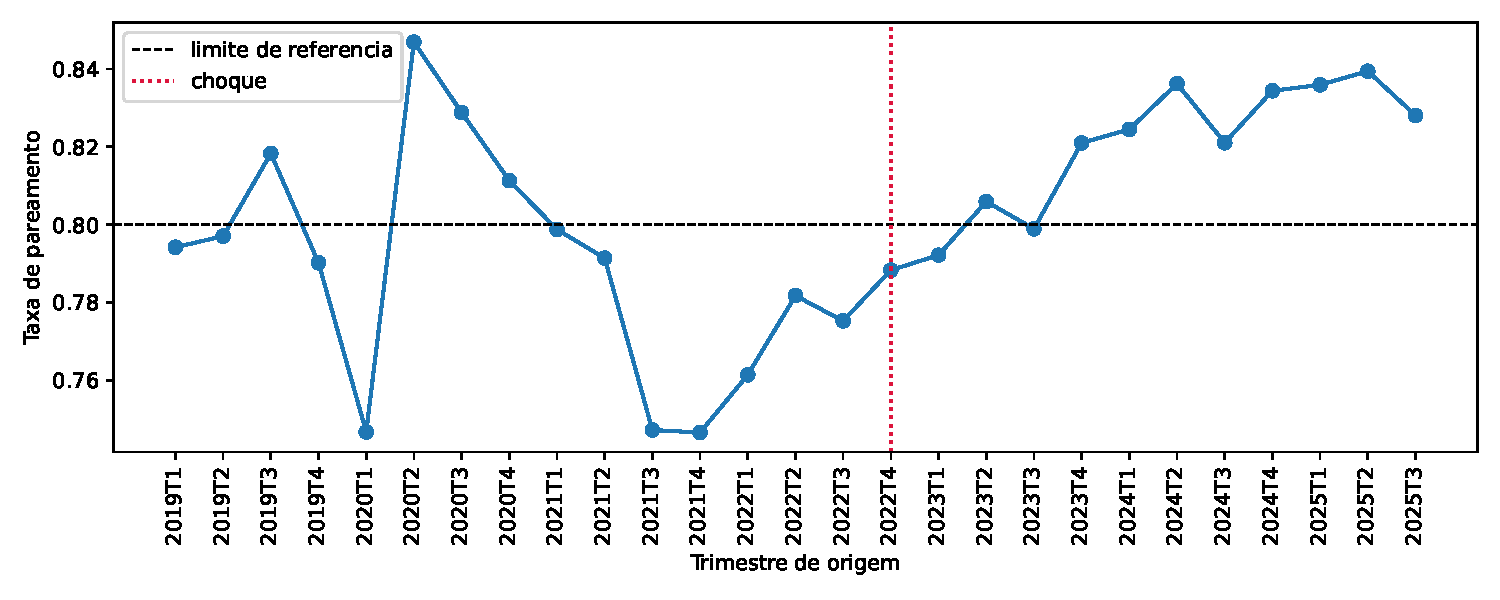
\includegraphics[width=0.92\textwidth]{figuras/fig_taxa_pareamento.pdf}
  \fonte{Elaboração própria a partir da PNADC/IBGE (2019T1--2025T3).}
  \nota{A linha de referência é 0,80. Os trimestres abaixo dela concentram-se no
        período de coleta atípica de 2020--2021.}
\end{figure}

\subsection{Filtragem da amostra}
\label{sec:filtragem}

A amostra analítica é obtida por uma sequência de cortes, todos justificados por
uma regra de desenho e nenhum por conveniência de resultado. A
Figura~\ref{fig:funil} apresenta o passo a passo com as quantidades efetivas em
cada etapa, medidas em pessoas-transições, isto é, na contagem de indivíduos
subjacente às células.

\begin{figure}[htbp]
  \caption{Passo a passo da filtragem dos dados, da PNADC aos domínios de estimação}
  \label{fig:funil}
  \centering
  \espacosimples
  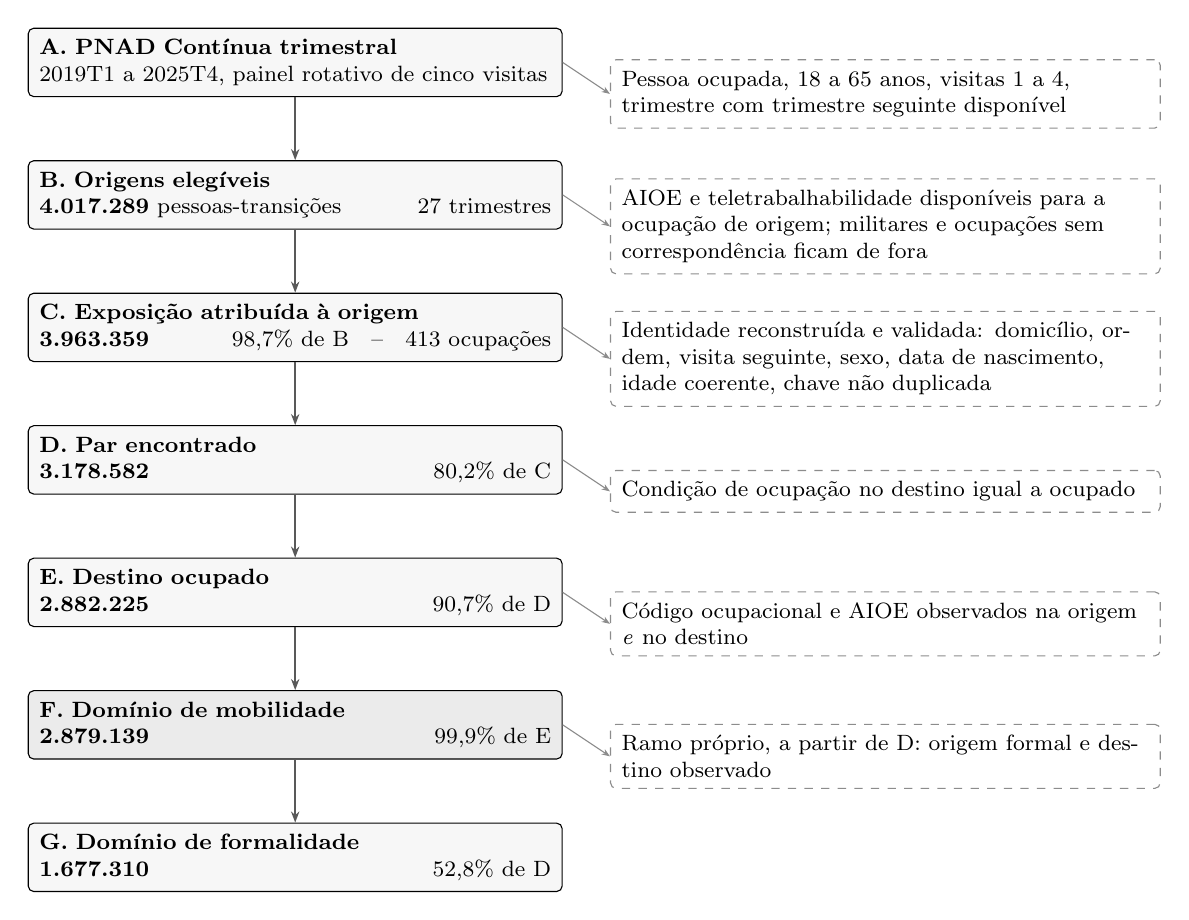
\begin{tikzpicture}[
      font=\fontsize{8}{9.6}\selectfont,
      caixa/.style={draw, rounded corners=2pt, align=left, inner sep=4pt,
                    text width=6.5cm, fill=black!3},
      corte/.style={draw=black!45, dashed, rounded corners=2pt, align=left,
                    inner sep=4pt, text width=6.7cm, fill=white},
      seta/.style={-{Stealth[length=4pt]}, thick, black!65},
      lig/.style={-{Stealth[length=3pt]}, black!45}
    ]
    \node[caixa] (a) {\textbf{A. PNAD Contínua trimestral}\\
      2019T1 a 2025T4, painel rotativo de cinco visitas};
    \node[caixa, below=8mm of a] (b) {\textbf{B. Origens elegíveis}\\
      \textbf{4.017.289} pessoas-transições \hfill 27 trimestres};
    \node[caixa, below=8mm of b] (c) {\textbf{C. Exposição atribuída à origem}\\
      \textbf{3.963.359} \hfill 98,7\% de B \; -- \; 413 ocupações};
    \node[caixa, below=8mm of c] (d) {\textbf{D. Par encontrado}\\
      \textbf{3.178.582} \hfill 80,2\% de C};
    \node[caixa, below=8mm of d] (e) {\textbf{E. Destino ocupado}\\
      \textbf{2.882.225} \hfill 90,7\% de D};
    \node[caixa, below=8mm of e, fill=black!8] (f) {\textbf{F. Domínio de mobilidade}\\
      \textbf{2.879.139} \hfill 99,9\% de E};
    \node[caixa, below=8mm of f] (g) {\textbf{G. Domínio de formalidade}\\
      \textbf{1.677.310} \hfill 52,8\% de D};

    \foreach \x/\y in {a/b, b/c, c/d, d/e, e/f, f/g} {\draw[seta] (\x) -- (\y);}

    \node[corte, right=6mm of a.east, anchor=west, yshift=-4mm] (ra)
      {Pessoa ocupada, 18 a 65 anos, visitas 1 a 4, trimestre com trimestre
       seguinte disponível};
    \node[corte, right=6mm of b.east, anchor=west, yshift=-4mm] (rb)
      {AIOE e teletrabalhabilidade disponíveis para a ocupação de origem;
       militares e ocupações sem correspondência ficam de fora};
    \node[corte, right=6mm of c.east, anchor=west, yshift=-4mm] (rc)
      {Identidade reconstruída e validada: domicílio, ordem, visita seguinte,
       sexo, data de nascimento, idade coerente, chave não duplicada};
    \node[corte, right=6mm of d.east, anchor=west, yshift=-4mm] (rd)
      {Condição de ocupação no destino igual a ocupado};
    \node[corte, right=6mm of e.east, anchor=west, yshift=-4mm] (re)
      {Código ocupacional e AIOE observados na origem \emph{e} no destino};
    \node[corte, right=6mm of f.east, anchor=west, yshift=-4mm] (rf)
      {Ramo próprio, a partir de D: origem formal e destino observado};

    \foreach \x/\y in {a/ra, b/rb, c/rc, d/rd, e/re, f/rf}
      {\draw[lig] (\x.east) -- (\y.west);}
  \end{tikzpicture}
  \fonte{Elaboração própria a partir da PNADC/IBGE.}
  \nota{As quantidades são pessoas-transições, não pessoas únicas: o mesmo
        indivíduo contribui com até quatro pares. Cada desfecho usa o domínio em
        que está definido: o teste de atrito usa todas as origens de C; a saída
        do emprego usa D; a mudança de ocupação usa E; as margens direcionais
        usam F; e a informalização usa G, que é um ramo lateral de D e não uma
        continuação de F.}
\end{figure}

Duas observações sobre a filtragem merecem destaque, porque afetam a leitura
dos resultados. Primeira: cada desfecho tem seu próprio domínio, e ausência
nunca é convertida em zero --- um destino não observado não é ``não mudou de
ocupação'', é simplesmente indefinido. Segunda: as quantidades são
pessoas-transições e não pessoas únicas, de modo que um mesmo indivíduo pode
contribuir com até quatro pares ao longo do painel, e os pesos amostrais somados
não são contagens de indivíduos independentes.

\subsection{Medida de exposição à inteligência artificial}
\label{sec:exposicao}

O tratamento é o \textit{Artificial Intelligence Occupational Exposure} (AIOE)
de \citeonline{felten2021}, publicado na classificação ocupacional americana
\textit{Standard Occupational Classification} de 2010 (SOC2010). A PNADC
classifica ocupação segundo a Classificação de Ocupações para Pesquisas
Domiciliares (COD), adaptação brasileira da \textit{International Standard
Classification of Occupations} de 2008 (ISCO-08). É necessária, portanto, uma
ponte em duas etapas: COD $\rightarrow$ ISCO-08 $\rightarrow$ SOC2010.

\subsubsection{Construção da ponte ocupacional}

A ponte é construída com resolução declarada elo a elo, e não por semelhança
numérica genérica:

\begin{enumerate}[label=\alph*)]
  \item grupos civis são comparados em quatro dígitos;
  \item o grupo 6 (agropecuária) é comparado em dois dígitos, porque o IBGE
        reagrupa esse bloco e a repartição fina seria arbitrária;
  \item entradas agregadas de três dígitos da correspondência oficial
        ISCO-SOC são incorporadas explicitamente;
  \item ocupações militares e o código 5168 não recebem exposição atribuída;
  \item entre os códigos SOC associados a um mesmo código COD, o peso é
        uniforme.
\end{enumerate}

A hipótese (e) é uma hipótese de construção declarada, não uma probabilidade
oficial de correspondência. Dos 434 códigos COD de quatro dígitos da estrutura
oficial, 427 recebem ao menos um elo, totalizando 1.148 elos, e o número máximo
de códigos SOC associados a um único COD é 37.

\subsubsection{Agregação da exposição para o código ocupacional}

Seja $S(c)$ o conjunto de códigos SOC ligados ao código ocupacional $c$, com
pesos $\omega_{cs} = 1/|S(c)|$. A exposição do código $c$ é a média ponderada

\begin{equation}
  A_c \;=\; \frac{\displaystyle\sum_{s \in S(c)} \omega_{cs} \, A_s \, \mathbb{1}\{A_s \text{ observado}\}}
                 {\displaystyle\sum_{s \in S(c)} \omega_{cs} \, \mathbb{1}\{A_s \text{ observado}\}},
  \label{eq:agregacao_exposicao}
\end{equation}

de modo que elos sem valor observado são \emph{ignorados} no cálculo, e não
tratados como zero --- tratá-los como zero introduziria atenuação mecânica
proporcional à incompletude da ponte. O mesmo procedimento é aplicado ao índice
de teletrabalhabilidade de \citeonline{dingel2020}, usado como controle.

A cobertura resultante é alta: 416 códigos COD recebem exposição e 413 recebem
também teletrabalhabilidade, sendo esses 413 os que entram na estimação. A
fração do peso amostral sem AIOE atribuído na origem é de 1,08\%, bem abaixo do
limite de 15\% fixado como critério de aceitação antes da estimação.

\subsubsection{Escala e padronização}

O AIOE é padronizado \emph{entre ocupações}, e não entre trabalhadores. Entre os
416 códigos COD com exposição, a média é 0,0053 e o desvio-padrão é
$\sigma_A = 0{,}9445$, praticamente unitário. Um coeficiente estimado ``por
unidade de AIOE'' lê-se, portanto, como ``por desvio-padrão de exposição entre
ocupações'', e é assim que todo coeficiente é reportado no
Capítulo~\ref{sec:resultados}. Ponderando por trabalhador, a média cai para
$-0{,}221$ e o desvio-padrão sobe para $0{,}981$: o emprego brasileiro
concentra-se em ocupações de exposição abaixo da média entre ocupações. A
Figura~\ref{fig:distribuicao} mostra a distribuição.

\begin{figure}[htb]
  \caption{Distribuição do AIOE entre códigos ocupacionais}
  \label{fig:distribuicao}
  \centering
  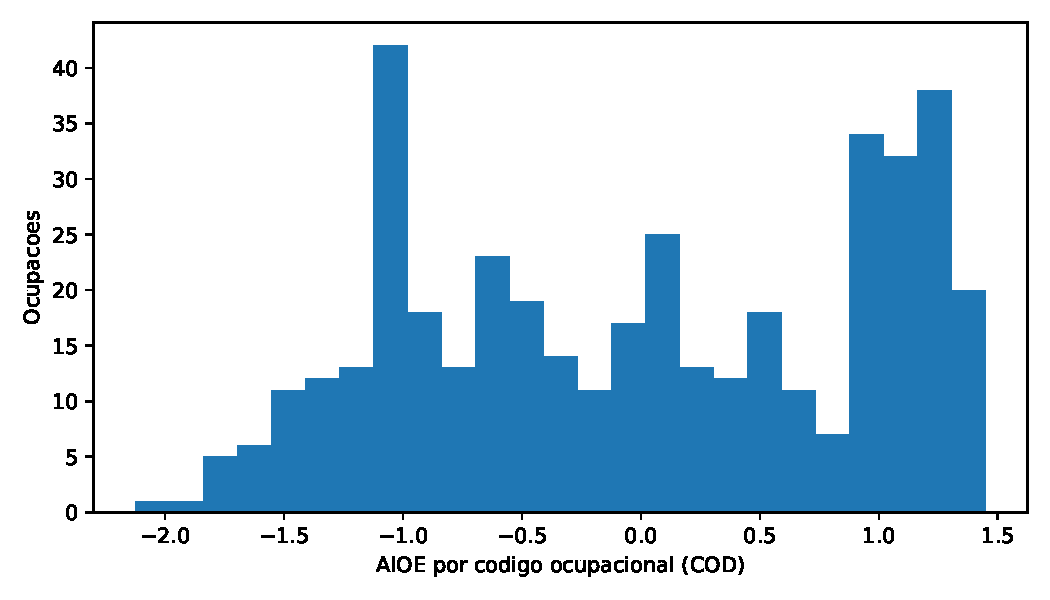
\includegraphics[width=0.85\textwidth]{figuras/fig_distribuicao_aioe.pdf}
  \fonte{Elaboração própria a partir de \citeonline{felten2021} e da PNADC/IBGE.}
\end{figure}

Uma segunda advertência de leitura decorre da escala e deve acompanhar todo
coeficiente reportado: AIOE menor significa \emph{menos exposição}, não emprego
pior, salário menor ou posição inferior na hierarquia ocupacional.

\subsubsection{Correlação com teletrabalhabilidade}

A correlação entre AIOE e teletrabalhabilidade entre códigos ocupacionais é de
$0{,}702$. Ocupações expostas à inteligência artificial são, em larga medida, as
mesmas ocupações que podem ser exercidas remotamente. Como o período analisado
contém a reorganização do trabalho remoto no pós-pandemia, omitir a
teletrabalhabilidade faria o coeficiente de exposição absorver essa
reorganização. Por isso o índice de teletrabalhabilidade entra na especificação
interagido com o indicador de período, exatamente na mesma forma funcional que o
tratamento.

\subsection{Definição dos desfechos}

São sete desfechos, organizados em três famílias e apresentados no
Quadro~\ref{qua:desfechos}. Seja $c(i)$ o código ocupacional de origem do par
$i$, $c'(i)$ o de destino, e $A_c$ a exposição da ocupação $c$ dada pela
equação~\eqref{eq:agregacao_exposicao}.

\begin{quadro}[htbp]
  \caption{Desfechos, definição formal e domínio de estimação}
  \label{qua:desfechos}
  \centering
  \espacosimples\idpcorpodez
  \begin{tabular}{@{}p{3.5cm}p{6.3cm}p{4.9cm}@{}}
    \toprule
    \textbf{Desfecho} & \textbf{Definição} & \textbf{Domínio} \\
    \midrule
    \multicolumn{3}{@{}l}{\textit{(i) Continuidade e vínculo}} \\
    \addlinespace[2pt]
    Pareamento
      & $1$ se a entrevista seguinte foi encontrada
      & todas as origens elegíveis \\
    Saída do emprego
      & $1$ se o destino não está ocupado
      & pares \\
    Formal para informal
      & $1$ se a origem é formal e o destino está ocupado e é informal
      & pares com origem formal e destino observado \\
    \addlinespace[3pt]
    \multicolumn{3}{@{}l}{\textit{(ii) Mobilidade ocupacional}} \\
    \addlinespace[2pt]
    Muda de ocupação (2 dígitos)
      & $1$ se $c'(i) \neq c(i)$ nos dois primeiros dígitos
      & pares com destino ocupado e ambos os códigos observados \\
    Muda de ocupação (3 dígitos)
      & $1$ se $c'(i) \neq c(i)$ nos três primeiros dígitos
      & idem \\
    \addlinespace[3pt]
    \multicolumn{3}{@{}l}{\textit{(iii) Deslocamento no gradiente de exposição}} \\
    \addlinespace[2pt]
    Mobilidade descendente
      & $1$ se $A_{c'(i)} < A_{c(i)}$
      & pares com AIOE observado nos dois lados \\
    Mobilidade ascendente
      & $1$ se $A_{c'(i)} > A_{c(i)}$
      & idem \\
    \bottomrule
  \end{tabular}
  \fonte{Elaboração própria (2026).}
\end{quadro}

A classificação de formalidade segue o dicionário oficial da pesquisa e não
admite código digitado à mão: empregado com carteira assinada, militar e
estatutário são formais; empregado sem carteira e trabalhador familiar auxiliar
são informais; conta-própria e empregador são classificados como formais
\emph{apenas} quando declaram inscrição no Cadastro Nacional da Pessoa Jurídica
(CNPJ), e ficam indefinidos quando a declaração está ausente. A escolha de
deixar indefinido em vez de imputar informalidade é deliberada: a alternativa
introduziria correlação espúria entre informalidade medida e não resposta.

O desfecho de pareamento cumpre função distinta das demais. Ele não é um
resultado de interesse substantivo, e sim um \textbf{teste de atrito}: se a
exposição da ocupação de origem previsse quem desaparece do painel, todos os
demais desfechos, definidos apenas sobre pares completos, estariam contaminados
por seleção. A leitura correta é a de um teste de falseamento, em que não
rejeitar é o resultado desejável.

O par de margens direcionais --- mobilidade descendente e ascendente --- é
sempre lido em conjunto, e nunca isoladamente. Quem parte de exposição alta só
pode se deslocar para baixo no gradiente, e vice-versa; a assimetria de nível é
mecânica e é absorvida pelo efeito fixo de ocupação, de modo que o contraste
informativo é a diferença entre os períodos, não o nível de cada margem.

\subsection{Análise descritiva}

A descrição precede e condiciona a estimação, e cobre dois blocos.

\subsubsection{Médias ponderadas por período}

Para cada desfecho calcula-se a média ponderada pelo peso amostral da origem no
período pré e no período pós, no domínio próprio daquele desfecho. Esse bloco
fixa a ordem de grandeza: antes de qualquer efeito diferencial, ele mostra
quanta rotatividade existe em um trimestre normal do mercado de trabalho
brasileiro, e permite julgar se um coeficiente de fração de ponto percentual é
grande ou pequeno em relação à margem que pretende explicar.

\subsubsection{Matriz de mobilidade entre faixas de exposição}

Os códigos ocupacionais são divididos em cinco faixas de exposição, com cortes
nos quintis da distribuição do AIOE \emph{entre códigos ocupacionais}, e não
entre trabalhadores. A escolha é deliberada: quintis definidos entre pessoas
seriam redefinidos pela própria recomposição do emprego, contaminando a
comparação entre períodos com a mudança que se pretende medir. As faixas são
fixas e idênticas no pré e no pós.

Para cada faixa de origem $q$ e cada faixa de destino $r$, calcula-se a
probabilidade ponderada de transição em cada período,

\begin{equation}
  \widehat{P}^{\,p}_{qr} \;=\;
  \frac{\displaystyle\sum_{i \in \mathcal{P}_p} w_i \, \mathbb{1}\{q_i = q, \, r_i = r\}}
       {\displaystyle\sum_{i \in \mathcal{P}_p} w_i \, \mathbb{1}\{q_i = q\}},
  \qquad p \in \{\text{pré}, \text{pós}\},
  \label{eq:matriz}
\end{equation}

e o objeto de interesse é a diferença $\widehat{D}_{qr} = \widehat{P}^{\,
\text{pós}}_{qr} - \widehat{P}^{\,\text{pré}}_{qr}$.

A incerteza vem de uma \textbf{reamostragem por unidade primária de amostragem}.
Em cada uma das 199 réplicas, sorteiam-se UPAs com reposição por um esquema
multinomial e a UPA inteira entra na réplica com suas observações pré e pós
conjuntas. Sortear o cluster inteiro, e não separadamente por período, preserva
tanto a correlação dentro da UPA quanto a dependência entre os dois períodos.

O teste de igualdade das matrizes pré e pós é um teste de Wald construído sobre
a matriz de covariância $\widehat{\Sigma}$ das réplicas. Empilhando as $25$
diferenças no vetor $\widehat{d}$,

\begin{equation}
  W \;=\; \widehat{d}^{\,\prime} \, \widehat{\Sigma}^{+} \, \widehat{d}
  \;\;\sim\;\; \chi^2_{\,\mathrm{posto}(\widehat{\Sigma})},
  \label{eq:wald}
\end{equation}

com $\widehat{\Sigma}^{+}$ denotando a pseudo-inversa de Moore-Penrose. O uso da
pseudo-inversa e dos graus de liberdade iguais ao posto é necessário porque as
linhas da matriz de transição somam um, o que torna $\widehat{\Sigma}$
singular por construção.

\subsection{Especificação econométrica}
\label{sec:espec}

\subsubsection{Desenho}

O desenho é de \textbf{diferenças em diferenças com tratamento contínuo}. Não há
grupo tratado e grupo de controle: há um marco temporal único e nacional --- o
lançamento público do ChatGPT, em 30 de novembro de 2022 --- e uma intensidade
de tratamento que varia entre ocupações, dada pela exposição da ocupação de
origem. O parâmetro de interesse é o \emph{gradiente} de resposta por
desvio-padrão de exposição, e não o efeito de um tratamento binário
\parencite{callaway2024}.

O indicador de período é definido no trimestre do marco:

\begin{equation}
  \text{Pós}_t =
  \begin{cases}
    1, & t \geq 2022\text{T}4, \\
    0, & t \leq 2022\text{T}3.
  \end{cases}
  \label{eq:pos}
\end{equation}

São, portanto, quinze trimestres de origem no período pré, de 2019T1 a 2022T3, e
doze no pós, de 2022T4 a 2025T3. O trimestre do marco é classificado como pós
por convenção declarada antes da estimação; ele contém dois meses anteriores ao
lançamento, e essa ambiguidade é registrada como limite conhecido, não corrigida
por exclusão.

\subsubsection{Equação estimada}

Para um par $i$ com ocupação de origem $c$, unidade da federação $u$ e trimestre
de origem $t$, estima-se

\begin{equation}
\begin{split}
  y_{icut} \;=\;{}& \beta \, \big( A_c \times \text{Pós}_t \big)
  \;+\; \gamma \, \big( T_c \times \text{Pós}_t \big)
  \;+\; \delta_1 \, \text{idade}_i + \delta_2 \, \text{idade}_i^2 \\[2pt]
  &+\; \alpha_c \;+\; \lambda_{ut} \;+\; \sum_{k \in \mathcal{K}} \theta^{k}_{g_k(i)}
  \;+\; \varepsilon_{icut},
\end{split}
  \label{eq:principal}
\end{equation}

em que $A_c$ é a exposição da ocupação de origem, $T_c$ é a sua
teletrabalhabilidade, $\alpha_c$ é o efeito fixo de ocupação de origem,
$\lambda_{ut}$ é o efeito fixo de UF interagida com trimestre de origem, e
$\mathcal{K}$ é o conjunto de efeitos fixos categóricos de sexo, cor ou raça,
escolaridade, categoria de tempo no emprego, categoria de tamanho do
estabelecimento e setor de atividade. Categorias ausentes recebem um nível
próprio, de modo que nenhuma célula é descartada silenciosamente. O coeficiente
de interesse é $\beta$, e a mesma especificação é aplicada, sem alteração, aos
sete desfechos.

Cada componente da equação~\eqref{eq:principal} tem função identificável:

\begin{enumerate}[label=\alph*)]
  \item $\alpha_c$ absorve o nível de cada ocupação. O coeficiente $\beta$ vem
        portanto da \emph{mudança de comportamento dentro} da ocupação ao longo
        do tempo, e não da comparação de níveis entre ocupações mais e menos
        expostas;
  \item $\lambda_{ut}$ absorve todo choque comum a uma UF em um trimestre,
        inclusive o ciclo macroeconômico nacional. Nenhum movimento comum a
        todo o país no período pode aparecer em $\beta$;
  \item $T_c \times \text{Pós}_t$ retira do coeficiente de exposição a
        reorganização do trabalho remoto, dada a correlação de $0{,}702$
        documentada na Seção~\ref{sec:exposicao};
  \item os efeitos fixos categóricos absorvem diferenças de composição
        demográfica e contratual que poderiam se confundir com exposição.
\end{enumerate}

\subsubsection{Ponderação e forma funcional}

A ponderação usa a soma do peso amostral da entrevista de \emph{origem}. Trata-se
de peso transversal, não de peso longitudinal calibrado para o painel: a PNADC
não publica peso longitudinal, e essa limitação é registrada na
Seção~\ref{sec:limites}.

Os desfechos binários são estimados por \textbf{modelo de probabilidade linear},
e não por modelo de resposta binária não linear. Duas razões. A primeira é de
viabilidade: a especificação contém efeitos fixos de alta dimensão, incluindo
mais de quatrocentos efeitos de ocupação e a interação completa de UF com
trimestre, e a estimação de modelos não lineares com essa estrutura enfrenta o
problema de parâmetros incidentais. A segunda é de alvo: o objeto de interesse é
o efeito marginal médio sobre a probabilidade de transição, que é diretamente o
coeficiente do modelo linear.

\subsection{Inferência}

O agrupamento dos erros-padrão é feito na \textbf{unidade primária de
amostragem}, que é o nível do desenho amostral da pesquisa e o nível em que a
correlação entre observações é mais evidente. O número de UPAs efetivamente
usadas varia entre 30.360 e 31.145 conforme o domínio do desfecho.

Os graus de liberdade são iguais ao número de grupos efetivamente usados menos
um, e os intervalos de confiança de 95\% são construídos pela distribuição $t$
com esses graus de liberdade, e não pela normal --- diferença imaterial com
mais de trinta mil grupos, mas registrada porque é o que o código faz.

Não há correção para multiplicidade de testes. São sete desfechos fortemente
correlacionados entre si, estimados sobre a mesma base e com a mesma
especificação; um valor-$p$ isolado de 0,03 não deve ser lido como achado forte,
e essa ressalva é feita no lugar de um ajuste formal.

\subsection{O que este desenho não identifica}
\label{sec:limites}

Esta seção é parte do método, não uma concessão retórica. Seis limites
delimitam o que pode ser afirmado.

\textbf{Primeiro: adoção de inteligência artificial não é observada.} O
tratamento é um índice de exposição ocupacional construído para a estrutura
ocupacional americana e transportado para a brasileira. Nenhuma empresa e
nenhum trabalhador da amostra é observado adotando qualquer ferramenta. O que se
mede é um gradiente associado à exposição potencial da ocupação.

\textbf{Segundo: o marco temporal é único e nacional.} Os efeitos fixos de UF
interagida com trimestre absorvem o que é comum, mas qualquer fator que tenha
atingido ocupações de alta exposição de forma diferencial no mesmo período ---
retomada pós-pandemia, difusão do trabalho remoto, ciclo setorial específico ---
entra no coeficiente. Não há variação exógena na intensidade do choque.

\textbf{Terceiro: não há bateria de robustez nesta versão.} O trabalho reporta
um único cenário de estimação. Janelas temporais alternativas, estruturas
alternativas de agrupamento, estudo de evento, testes de tendência pré-marco e
análise formal de sensibilidade a violações de paralelismo não são executados
aqui, e o Capítulo~\ref{sec:melhorias} organiza essa agenda. Enquanto ela não for
executada, a leitura correta dos coeficientes é a de \emph{associação
condicional}, não a de efeito causal.

\textbf{Quarto: a seleção longitudinal permanece.} O peso é transversal e não há
correção de atrito. O teste de pareamento limita, mas não elimina, a
preocupação: ele detecta seleção associada à exposição, não seleção por
características não observadas.

\textbf{Quinto: o horizonte é de um trimestre.} Realocação lenta, mudança de
carreira, requalificação e efeitos sobre a entrada no mercado de trabalho não
aparecem nesta margem.

\textbf{Sexto: direção de exposição não é bem-estar.} Deslocar-se para uma
ocupação de menor AIOE significa menor exposição à inteligência artificial, e
não menor salário, pior contrato ou perda de posição.

Uma observação adicional, de natureza temporal, fecha o capítulo. As covariáveis
e a exposição pertencem à origem de cada par, e as origens do período pós podem
refletir escolhas ocupacionais já influenciadas pelo próprio marco. Não se trata,
portanto, de atribuição fixa de tratamento em uma linha de base anterior a 2022,
e sim de exposição contemporânea à origem de cada transição.

\section{Resultados preliminares}
\label{sec:resultados}

Este capítulo apresenta os resultados obtidos até o momento. O adjetivo
``preliminares'' é literal e tem duas justificativas. A primeira é que o trabalho
reporta, nesta versão, um \emph{único} cenário de estimação: a especificação da
equação~\eqref{eq:principal}, com o corte de período no trimestre do marco e
erros-padrão agrupados por unidade primária de amostragem. Não há aqui bateria
de sensibilidade, estudo de evento nem teste formal de tendências pré-marco, de
modo que os coeficientes devem ser lidos como \textbf{associação condicional}, e
não como estimativas causais do efeito do marco. A segunda é que a agenda de
robustez descrita no Capítulo~\ref{sec:melhorias} (medidas alternativas de
exposição, estimadores alternativos e tratamento do problema de coleta) ainda
não foi executada. O capítulo organiza-se em três blocos: descrição da amostra e
das margens de transição; resultado principal; e síntese.

\subsection{Descrição da amostra e das margens de transição}

A Tabela~\ref{tab:escala} apresenta a escala efetiva de cada domínio de
estimação. O ponto de partida são 3.963.359 pessoas-transições com exposição
atribuída à ocupação de origem, distribuídas por 413 códigos ocupacionais,
31.145 unidades primárias de amostragem e 27 trimestres de origem. Cada desfecho
usa o subconjunto em que está definido, e nenhuma ausência é convertida em zero.

% Gerado por scripts/06_dissertacao.py a partir de output/modelos e output/tabelas.
% Não editar à mão: a próxima execução sobrescreve este arquivo.
\begin{table}[htb]
  \caption{Escala dos domínios de estimação}
  \label{tab:escala}
  \centering
  \espacosimples\idpcorpodez
  \begin{tabular}{@{}lrrrr@{}}
    \toprule
    \textbf{Domínio (desfecho)}                & \textbf{Pessoas-} & \textbf{Células} & \textbf{Ocupa-} & \textbf{UPAs} \\
                                               & \textbf{transições} & \textbf{estimadas} & \textbf{ções} & \\
    \midrule
    Todas as origens (pareamento)              & 3.963.359    & 3.960.584    & 413        & 31.145 \\
    Pares (saída do emprego)                   & 3.178.582    & 3.176.283    & 413        & 31.047 \\
    Destino ocupado (muda de ocupação)         & 2.882.225    & 2.880.049    & 413        & 31.036 \\
    AIOE nos dois lados (margens direcionais)  & 2.879.139    & 2.876.964    & 413        & 31.036 \\
    Origem formal (informalização)             & 1.677.310    & 1.676.862    & 411        & 30.360 \\
    \bottomrule
  \end{tabular}
  \fonte{Elaboração própria a partir da PNADC/IBGE.}
  \nota{Origens de 2019T1 a 2025T3. Pessoas-transições não são pessoas únicas: o
        mesmo indivíduo contribui com até quatro pares. A coluna de células é o
        número de observações efetivamente estimadas em cada modelo.}
\end{table}


A Tabela~\ref{tab:descritivas} traz as médias ponderadas antes e depois do
marco. Três leituras importam. Primeira: as margens direcionais de exposição
sobem quase na mesma proporção (a mobilidade descendente passa de 12,8\% para
17,4\% e a ascendente, de 12,9\% para 17,4\%), o que é compatível com aumento geral das taxas medidas de rotatividade
ocupacional, e não com deslocamento líquido do emprego para ocupações menos
expostas. Segunda: a mudança de ocupação sobe entre sete e oito pontos
percentuais nas duas resoluções, reforçando essa leitura. Terceira: a transição
de formal para informal aumenta cerca de 69\%, de 5,2\% para 8,8\%, movimento
de grande magnitude que exige leitura conjunta
com o ciclo do mercado de trabalho no período. A saída do emprego, em contraste,
praticamente não se move.

% Gerado por scripts/06_dissertacao.py a partir de output/modelos e output/tabelas.
% Não editar à mão: a próxima execução sobrescreve este arquivo.
\begin{table}[htb]
  \caption{Médias ponderadas dos desfechos, antes e depois do marco}
  \label{tab:descritivas}
  \centering
  \espacosimples\idpcorpodez
  \begin{tabular}{@{}lrrr@{}}
    \toprule
    \textbf{Desfecho}                     & \textbf{Pré} & \textbf{Pós} & \textbf{Diferença} \\
    \midrule
    \multicolumn{4}{@{}l}{\textit{Continuidade e vínculo}} \\
    Pareamento entre entrevistas          & 0,783 & 0,812 & $+$0,029 \\
    Saída do emprego                      & 0,079 & 0,081 & $+$0,002 \\
    Transição de formal para informal     & 0,052 & 0,088 & $+$0,036 \\
    \addlinespace
    \multicolumn{4}{@{}l}{\textit{Mobilidade ocupacional}} \\
    Muda de ocupação (2 dígitos)          & 0,209 & 0,280 & $+$0,071 \\
    Muda de ocupação (3 dígitos)          & 0,236 & 0,318 & $+$0,082 \\
    \addlinespace
    \multicolumn{4}{@{}l}{\textit{Gradiente de exposição}} \\
    Transição para menor AIOE             & 0,128 & 0,174 & $+$0,046 \\
    Transição para maior AIOE             & 0,129 & 0,174 & $+$0,046 \\
    \bottomrule
  \end{tabular}
  \fonte{Elaboração própria a partir da PNADC/IBGE.}
  \nota{Pré: origens de 2019T1 a 2022T3. Pós: origens de 2022T4 a 2025T3, pelo
        corte da equação~\eqref{eq:pos}. Médias ponderadas pelo peso amostral da
        entrevista de origem, cada uma no domínio próprio do desfecho.}
\end{table}


A Tabela~\ref{tab:matriz} apresenta a diferença entre as matrizes de mobilidade
pós e pré entre faixas de exposição. O padrão é inequívoco e não é um padrão de
direção: \emph{a permanência na mesma faixa cai em todas as cinco faixas}, entre
3,6 e 8,1 pontos percentuais, com a queda mais forte na quarta faixa. O teste de
Wald da equação~\eqref{eq:wald} rejeita a igualdade das matrizes com estatística
de 3.040,1 e 20 graus de liberdade. A Figura~\ref{fig:matriz} apresenta a mesma
informação em forma gráfica.

% Gerado por scripts/06_dissertacao.py a partir de output/modelos e output/tabelas.
% Não editar à mão: a próxima execução sobrescreve este arquivo.
\begin{table}[htb]
  \caption{Diferença entre as matrizes de mobilidade pós e pré, por faixa de exposição}
  \label{tab:matriz}
  \centering
  \espacosimples\idpcorpodez
  \begin{tabular}{@{}lrrrrr@{}}
    \toprule
    \textbf{Faixa de origem} & \multicolumn{5}{c}{\textbf{Faixa de destino (p.p.)}} \\
    \cmidrule(l){2-6}
     & \textbf{Q1} & \textbf{Q2} & \textbf{Q3} & \textbf{Q4} & \textbf{Q5} \\
    \midrule
    Q1 (menor exposição) & $-$3,60  & $+$2,03  & $+$1,04  & $+$0,34  & $+$0,19 \\
    Q2                   & $+$2,05  & $-$4,97  & $+$1,60  & $+$0,75  & $+$0,57 \\
    Q3                   & $+$1,17  & $+$1,83  & $-$6,42  & $+$1,55  & $+$1,87 \\
    Q4                   & $+$0,69  & $+$1,22  & $+$2,46  & $-$8,06  & $+$3,69 \\
    Q5 (maior exposição) & $+$0,26  & $+$0,82  & $+$1,92  & $+$2,78  & $-$5,79 \\
    \bottomrule
  \end{tabular}
  \fonte{Elaboração própria a partir da PNADC/IBGE.}
  \nota{Faixas fixas entre códigos ocupacionais. Erros-padrão por reamostragem
        de UPA (199 réplicas) variam entre 0,04 e 0,28 p.p.; todas as células
        têm intervalo de 95\% que exclui zero. Teste de Wald de igualdade das
        matrizes: $\chi^2 = 3.040{,}1$, 20 graus de liberdade.}
\end{table}


\begin{figure}[htb]
  \caption{Diferença entre as matrizes de mobilidade pós e pré}
  \label{fig:matriz}
  \centering
  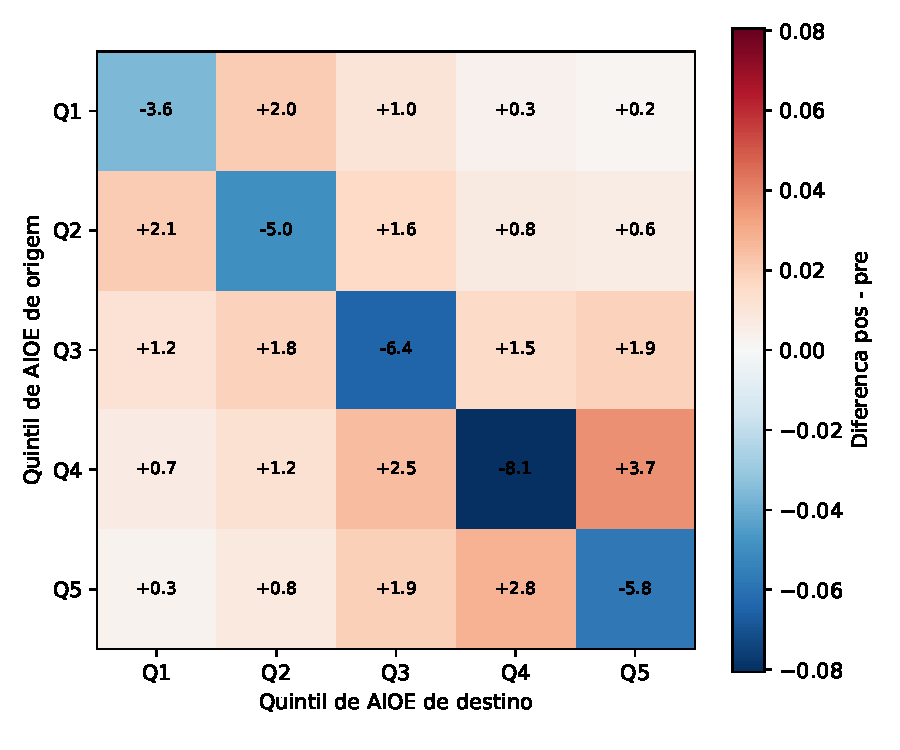
\includegraphics[width=0.85\textwidth]{figuras/fig_matriz_diferencas.pdf}
  \fonte{Elaboração própria a partir da PNADC/IBGE.}
\end{figure}

Um achado descritivo adicional merece registro porque condiciona toda a leitura
temporal. A taxa ponderada de mudança de código ocupacional em três dígitos
entre entrevistas consecutivas cai abruptamente de 30,0\% nas origens de 2019T4
para 15,3\% nas de 2020T1, permanece entre 13\% e 15\% durante todo o período de
coleta telefônica e retorna a 34,3\% nas origens de 2021T4. Essa
descontinuidade coincide com as mudanças no modo de coleta da pesquisa
\parencite{ibge2022tratamento}, o que torna plausível um problema de medida. Os
dados aqui apresentados, porém, não separam o efeito da coleta de mudanças reais
do mercado de trabalho na pandemia, de alterações de composição amostral, do
atrito e da codificação ocupacional. Tampouco a comparação entre a magnitude
dessa quebra agregada e a dos coeficientes demonstra, por si, viés no gradiente:
para isso seria preciso verificar se a quebra varia com a exposição. Como o
desenho desta versão usa a série inteira, parte do contraste entre pré e pós
atravessa essa descontinuidade, razão pela qual seu tratamento encabeça a agenda
do Capítulo~\ref{sec:melhorias}.

\subsection{Resultado principal}

A Tabela~\ref{tab:principal} apresenta os coeficientes da
equação~\eqref{eq:principal} para os sete desfechos, em pontos percentuais por unidade de AIOE da ocupação de origem (cerca de um
desvio-padrão entre ocupações; Seção~\ref{sec:exposicao}). O painel A traz o coeficiente
de interesse $\beta$, sobre a interação entre exposição e período; o painel B
traz o coeficiente $\gamma$ da teletrabalhabilidade interagida com o período,
estimado simultaneamente na mesma equação. A Figura~\ref{fig:coeficientes}
apresenta o painel A em forma gráfica.

% Gerado por scripts/06_dissertacao.py a partir de output/modelos e output/tabelas.
% Não editar à mão: a próxima execução sobrescreve este arquivo.
\begin{table}[htb]
  \caption{Gradiente de exposição e de teletrabalhabilidade, cenário único}
  \label{tab:principal}
  \centering
  \espacosimples\idpcorpodez
  \begin{tabular}{@{}lrrlr@{}}
    \toprule
    \textbf{Desfecho}                  & \textbf{Efeito (p.p.)} & \textbf{E.P.} & \textbf{IC 95\%}       & \textbf{$p$} \\
    \midrule
    \multicolumn{5}{@{}l}{\textit{Painel A --- Exposição $\times$ pós}} \\
    \addlinespace[2pt]
    Transição para menor AIOE          & $+$2,187  & 0,105 & [$+$1,982; $+$2,393]   & $<$0,001 \\
    Muda de ocupação (3 dígitos)       & $+$0,861  & 0,136 & [$+$0,594; $+$1,128]   & $<$0,001 \\
    Muda de ocupação (2 dígitos)       & $+$0,278  & 0,128 & [$+$0,027; $+$0,529]   & 0,030 \\
    Saída do emprego                   & $-$0,250  & 0,075 & [$-$0,398; $-$0,103]   & $<$0,001 \\
    Pareamento (teste de atrito)       & $-$0,261  & 0,141 & [$-$0,536; $+$0,015]   & 0,064 \\
    Transição de formal para informal  & $-$0,673  & 0,094 & [$-$0,858; $-$0,488]   & $<$0,001 \\
    Transição para maior AIOE          & $-$1,364  & 0,103 & [$-$1,566; $-$1,161]   & $<$0,001 \\
    \addlinespace
    \multicolumn{5}{@{}l}{\textit{Painel B --- Teletrabalhabilidade $\times$ pós}} \\
    \addlinespace[2pt]
    Transição para menor AIOE          & $-$0,239  & 0,255 & [$-$0,739; $+$0,262]   & 0,350 \\
    Muda de ocupação (3 dígitos)       & $+$0,093  & 0,309 & [$-$0,512; $+$0,698]   & 0,763 \\
    Muda de ocupação (2 dígitos)       & $+$0,391  & 0,290 & [$-$0,178; $+$0,960]   & 0,178 \\
    Saída do emprego                   & $+$0,215  & 0,153 & [$-$0,086; $+$0,515]   & 0,161 \\
    Pareamento (teste de atrito)       & $-$0,362  & 0,291 & [$-$0,932; $+$0,208]   & 0,213 \\
    Transição de formal para informal  & $+$1,734  & 0,199 & [$+$1,345; $+$2,124]   & $<$0,001 \\
    Transição para maior AIOE          & $+$0,762  & 0,221 & [$+$0,330; $+$1,195]   & $<$0,001 \\
    \bottomrule
  \end{tabular}
  \fonte{Elaboração própria a partir da PNADC/IBGE.}
  \nota{Efeito em pontos percentuais por desvio-padrão de exposição da ocupação
        de origem, no painel A, e por unidade do índice de teletrabalhabilidade,
        no painel B. Os dois painéis vêm da mesma estimação. Erros-padrão
        agrupados por UPA, entre 30.360 e 31.145 grupos conforme o domínio. O
        desfecho de pareamento é um teste de atrito: não rejeitar é o resultado
        desejável.}
\end{table}


\begin{figure}[htb]
  \caption{Gradiente de exposição por desfecho, com intervalos de 95\%}
  \label{fig:coeficientes}
  \centering
  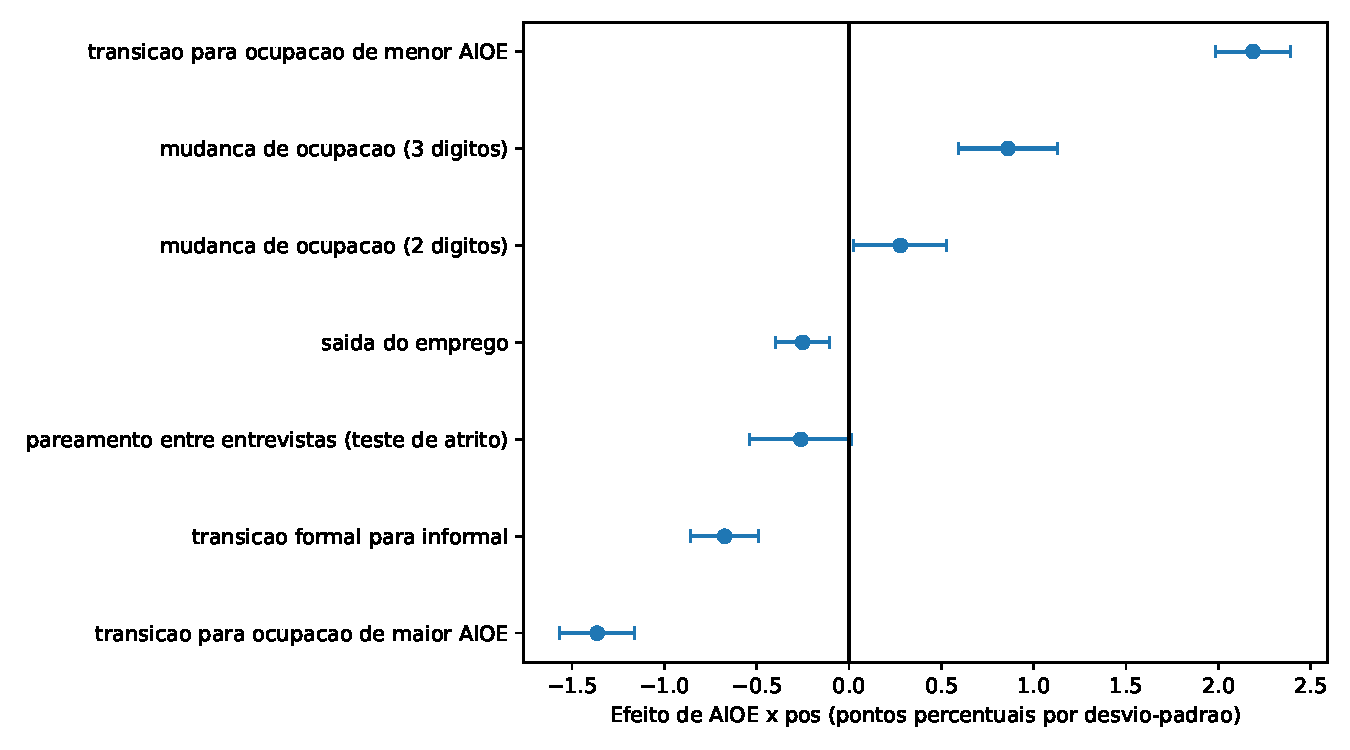
\includegraphics[width=0.92\textwidth]{figuras/fig_coeficientes_aioe.pdf}
  \fonte{Elaboração própria a partir da PNADC/IBGE.}
  \nota{Efeito da interação entre exposição e período, em pontos percentuais por
        unidade de AIOE da ocupação de origem.}
\end{figure}

A leitura literal é a seguinte. Condicionalmente aos efeitos fixos de ocupação
de origem e de UF-trimestre, à teletrabalhabilidade interagida com o período e
ao conjunto de covariáveis demográficas e contratuais, a mudança entre o período
pré e o pós na probabilidade de transitar para ocupação menos exposta é 2,19
pontos percentuais maior para ocupações de origem com uma unidade a mais de
AIOE; na probabilidade de transitar para ocupação mais exposta, a mudança é 1,36
ponto percentual menor. O coeficiente compara, portanto, as mudanças entre pré e
pós de ocupações com exposições diferentes, e não acompanha uma mesma ocupação
cuja exposição aumente, já que o AIOE é constante dentro de cada ocupação.

Esses dois números precisam ser lidos em conjunto e contra o pano de fundo
descritivo. As duas margens direcionais subiram \emph{ambas} cerca de 4,6 pontos
percentuais entre os períodos, conforme a Tabela~\ref{tab:descritivas}. O que os
coeficientes acrescentam é que essa subida geral não foi simétrica ao longo do
gradiente: entre ocupações de origem, quanto maior a exposição, mais a
composição do movimento pendeu para o lado descendente. Essa assimetria, porém,
não é necessariamente específica à exposição: como discutido na
Seção~\ref{sec:desfechos}, origens mais expostas têm mais destinos possíveis
abaixo delas, e um aumento geral de mobilidade tende, por si só, a elevar mais
sua mobilidade descendente, canal que o desenho atual não separa do gradiente.
Em magnitude, o coeficiente corresponde a cerca de 12,6\% da taxa pós de
transição para ocupação menos exposta (2,19 pontos percentuais sobre 17,4\%).

O terceiro grupo de resultados é o de frequência de mudança. Maior exposição
associa-se a mais mudança de ocupação, com $+0{,}86$ ponto percentual na
resolução de três dígitos e $+0{,}28$ na de dois dígitos. A diferença entre as duas resoluções sugere que parte do movimento adicional
associado à exposição ocorre \emph{dentro} das categorias de dois dígitos da
COD, e não entre elas; uma inferência formal sobre essa diferença exigiria
considerar a covariância entre as duas estimativas.

O quarto grupo é o das margens de vínculo, e o sinal é contraintuitivo. Maior
exposição associa-se a \emph{menos} saída do emprego ($-0{,}25$ ponto
percentual) e a \emph{menos} transição de formal para informal ($-0{,}67$ ponto
percentual). Isto é, no período analisado, trabalhadores em ocupações mais
expostas não apresentaram deterioração relativa de vínculo; se algo, o contrário.
Nesse desfecho, o coeficiente da teletrabalhabilidade é positivo e expressivo
($+1{,}73$ ponto percentual por unidade do índice, painel B), enquanto o da
exposição é negativo. Como os dois índices têm escalas distintas, os
coeficientes não são diretamente comparáveis em magnitude: o desenho permite
relatar os dois gradientes condicionais, mas não identificar qual força explica
o aumento agregado da informalização.

O teste de atrito merece nota específica. O coeficiente sobre a probabilidade de
pareamento é $-0{,}261$ ponto percentual, com $p = 0{,}064$: não se rejeita a hipótese de que o gradiente de pareamento em relação à
exposição tenha permanecido estável entre os períodos, mas o resultado está
próximo do limiar convencional e o sinal é negativo. Como diferenças
permanentes de retenção entre ocupações são absorvidas pelo efeito fixo, o teste
também não as avalia. Isso não invalida os demais desfechos, mas impede afirmar
que a seleção longitudinal esteja descartada.

Uma ressalva de leitura fecha a seção. São sete desfechos fortemente
correlacionados, estimados sobre a mesma base e com a mesma especificação, sem
correção para multiplicidade. O coeficiente de mudança de ocupação em dois
dígitos, com $p = 0{,}030$, é o que menos resiste a essa ressalva e não deve ser
citado isoladamente.

\subsection{Síntese dos resultados preliminares}

Os resultados preliminares sustentam quatro afirmações, e apenas quatro.

\textbf{Primeira.} Houve aumento generalizado das taxas medidas de rotatividade
ocupacional na amostra entre o período pré e o pós, visível na queda de
permanência em \emph{todas} as faixas de exposição e na subida simultânea das
duas margens direcionais. Parte relevante desse movimento é comum às ocupações,
o que não exclui a participação de mecanismos associados à exposição.

\textbf{Segunda.} Condicionalmente à ocupação de origem, ao par UF-trimestre, à
teletrabalhabilidade interagida com o período e ao conjunto de controles, há
gradiente estatisticamente detectável associado à exposição: maior exposição
associa-se a mais transições para ocupações menos expostas, menos transições
para ocupações mais expostas e mais mudança de ocupação, sobretudo de resolução
fina. A magnitude é da ordem de dois pontos percentuais por unidade de AIOE, cerca
de um oitavo da taxa pós de transição para ocupação menos exposta. Nas margens
direcionais, esse gradiente não está separado do canal mecânico descrito na
Seção~\ref{sec:desfechos}.

\textbf{Terceira.} Nas margens de vínculo o sinal é o oposto do que a leitura
alarmista sobre inteligência artificial anteciparia: maior exposição associa-se a
menos saída do emprego e a menos informalização. Na informalização, o gradiente é negativo em relação à exposição e positivo em
relação à teletrabalhabilidade, sem que o desenho identifique qual força explica
o aumento agregado.

\textbf{Quarta, e limitante.} Nada disso é evidência causal. O desenho reporta um
único cenário, sem estudo de evento, sem teste de tendências pré-marco e sem
bateria de sensibilidade; a série usada atravessa uma descontinuidade na taxa medida de mudança de
ocupação em 2020 e 2021, coincidente com a mudança no modo de coleta e de causa
ainda não demonstrada. Os coeficientes da Tabela~\ref{tab:principal}
devem ser lidos como descrição condicional de um período que contém essa
descontinuidade. O Capítulo~\ref{sec:melhorias} organiza o que precisa ser feito
para mudar esse diagnóstico, e coloca o tratamento do problema de coleta como
prioridade.

\section{Considerações e melhorias posteriores}
\label{sec:melhorias}

Este capítulo cumpre duas funções. Na primeira seção, retoma a pergunta de
pesquisa e sintetiza o que os resultados preliminares do
Capítulo~\ref{sec:resultados} permitem e não permitem afirmar. Nas seções
seguintes, organiza a agenda de melhorias posteriores em quatro frentes ---
medidas alternativas de exposição, técnicas econométricas alternativas,
tratamento do problema de medida na coleta da pesquisa e extensões de escopo ---
com a indicação, em cada caso, de qual limitação específica a melhoria pretende
resolver.

\subsection{Considerações sobre os resultados obtidos}

A pergunta de pesquisa é se trabalhadores em ocupações mais expostas à
inteligência artificial passaram a apresentar transições de trabalho distintas
após o lançamento público do ChatGPT. A resposta que os dados sustentam hoje é
qualificada em três níveis.

No nível descritivo, a resposta é que houve mudança generalizada, e não
mudança concentrada nas ocupações expostas. A permanência na mesma faixa de
exposição caiu entre 3,6 e 8,1 pontos percentuais em todas as cinco faixas, e as
margens de mobilidade ascendente e descendente subiram quase na mesma proporção.
O mercado de trabalho brasileiro ficou mais móvel no período; a exposição
ocupacional não explica esse movimento agregado.

No nível de associação condicional, a resposta é que existe um gradiente
detectável, porém modesto. Controlada a ocupação de origem, o par UF-trimestre,
a teletrabalhabilidade interagida com o período e o conjunto de covariáveis, um
desvio-padrão adicional de exposição associa-se a aproximadamente 2,2 pontos
percentuais a mais de transição para ocupação menos exposta e a 1,4 ponto
percentual a menos de transição para ocupação mais exposta. Nas margens de
vínculo o sinal é o inverso do esperado pela leitura alarmista: maior exposição
associa-se a menos saída do emprego e a menos informalização, e a informalização
do período aparece associada à teletrabalhabilidade, não à exposição.

No nível causal, a resposta é que o desenho atual não sustenta a afirmação, por
duas razões de natureza distinta. A primeira é de escopo: esta versão do
trabalho reporta um único cenário de estimação, sem estudo de evento, sem teste
de tendências pré-marco e sem bateria de sensibilidade. Um coeficiente que não
foi submetido a esses testes não pode ser apresentado como efeito causal,
qualquer que seja o seu valor-$p$. A segunda é de medida, e é a mais séria: a
taxa medida de mudança de ocupação cai pela metade durante os trimestres de
coleta telefônica de 2020 e 2021 e volta ao patamar anterior em 2021T4, uma
descontinuidade maior que qualquer coeficiente estimado aqui e que atravessa o
período pré. Enquanto ela não for tratada, todo contraste entre pré e pós que
use a série inteira é, em parte, contraste entre modos de coleta. É esse fato
que organiza toda a agenda a seguir e que promove o tratamento do problema de
coleta de item de robustez a prioridade.

\subsection{Medidas alternativas de exposição à inteligência artificial}
\label{sec:exposicoes}

A primeira frente de robustez ataca a validade da variável de tratamento. Hoje
o trabalho depende de uma única medida, o AIOE de \citeonline{felten2021},
construída para a classificação ocupacional americana, anterior à difusão dos
modelos generativos e transportada para a classificação brasileira por uma ponte
com pesos uniformes declarados. Cada uma dessas três características é uma
hipótese que pode falhar, e a maneira de testá-las é substituir a medida
mantendo tudo o mais constante.

\subsubsection{Exposição específica a modelos de linguagem}

A substituição mais direta é pela medida de \citeonline{eloundou2024},
construída tarefa a tarefa para modelos de linguagem de grande porte e
contemporânea ao marco temporal usado aqui. Ela responde à objeção mais óbvia
que o trabalho atual atrai: o AIOE mede exposição à inteligência artificial em
sentido amplo, incluindo visão computacional e reconhecimento de padrões, que
não são a tecnologia cujo lançamento define o marco. Se o gradiente estimado com
a medida específica for maior que o estimado com a medida ampla, isso é evidência
a favor da leitura pretendida; se for menor ou nulo, é evidência de que o
gradiente atual capta outra coisa.

\subsubsection{Exposição por conteúdo de tarefas rotineiras e não rotineiras}

Uma segunda substituição usa medidas de conteúdo de tarefas, na tradição de
\citeonline{acemoglu2020}, para separar exposição a automação de rotinas de
exposição a automação de tarefas cognitivas. Essa distinção é a que dá sentido
econômico à direção prevista do efeito e permite testar se o gradiente estimado
é específico à dimensão cognitiva ou se reflete simplesmente rotinização.

\subsubsection{Teletrabalhabilidade como tratamento placebo}

Dada a correlação de $0{,}702$ entre exposição e teletrabalhabilidade, um
exercício informativo é inverter os papéis: estimar a mesma especificação usando
a teletrabalhabilidade como tratamento e a exposição como controle. Se o
gradiente de teletrabalhabilidade for da mesma ordem de grandeza, a
interpretação em termos de inteligência artificial fica insustentável e o
resultado passa a ser sobre reorganização do trabalho remoto.

\subsubsection{Sensibilidade à construção da ponte ocupacional}

A ponte COD-ISCO-SOC usa pesos uniformes entre códigos SOC associados ao mesmo
código COD, comparação em dois dígitos no grupo da agropecuária e ausência de
atribuição a ocupações militares. Convém reestimar com pontes alternativas ---
pesos proporcionais ao emprego americano por SOC, comparação em três dígitos
para todos os grupos, e restrição da amostra aos códigos COD com correspondência
unívoca --- para medir quanto do resultado depende dessas escolhas de
construção.

\subsubsection{Exposição medida no destino, e não só na origem}

Por fim, todas as covariáveis e a exposição pertencem hoje à origem do par. Uma
extensão natural é modelar a exposição do destino como escolha, o que
transformaria o problema de um gradiente de transição em um modelo de escolha
ocupacional com exposição como atributo da alternativa.

\subsection{Técnicas econométricas alternativas}

A segunda frente ataca a identificação. O procedimento atual é um modelo de
probabilidade linear com interação entre tratamento contínuo e indicador de
período, estimado com efeitos fixos de alta dimensão. Essa escolha é defensável,
mas está longe de ser a única, e os problemas diagnosticados no
Capítulo~\ref{sec:resultados} pedem estimadores construídos justamente para
tratar deles.

\subsubsection{Diferenças em diferenças com tratamento contínuo}

O estimador atual impõe, implicitamente, que a resposta seja linear na dose de
exposição e que a comparação entre doses diferentes seja livre de seleção.
\citeonline{callaway2024} mostram que essa hipótese é mais forte do que parece e
propõem parâmetros e estimadores que separam o efeito médio em cada nível de dose
da comparação entre níveis. Aplicar esse arcabouço permitiria responder se o
gradiente estimado é um efeito de dose ou um artefato de composição entre
ocupações com doses diferentes.

\subsubsection{Análise formal de sensibilidade a tendências não paralelas}

O passo anterior a qualquer análise formal de sensibilidade é o estudo de
evento: substituir a interação única com o indicador de período por interações
com cada trimestre relativo ao marco, examinar se os coeficientes pré são planos
e submetê-los a teste conjunto. Feito isso, a análise de
\citeonline{rambachan2023} responde à pergunta seguinte --- qual é a menor
violação de paralelismo no período pós, expressa como múltiplo do maior desvio
pré observado, capaz de fazer o intervalo de confiança passar a incluir zero. A
melhoria consiste em executar os dois e reportar, para cada desfecho, o
intervalo robusto em vez do intervalo convencional, discutindo qual magnitude de
violação é economicamente plausível dado o que se sabe sobre a coleta da
pesquisa.

\subsubsection{Grupos de comparação construídos por pareamento}

Uma alternativa ao controle por efeitos fixos é construir explicitamente um
contrafactual: parear ocupações de alta exposição com ocupações de baixa
exposição semelhantes em trajetória pré-marco, escolaridade média, composição
setorial e teletrabalhabilidade, e estimar a diferença apenas entre pares
comparáveis. Métodos de controle sintético aplicados a séries ocupacionais
agregadas seguem a mesma lógica e têm a vantagem de tornar visível a qualidade
do ajuste pré-marco, que é exatamente o ponto fraco do desenho atual.

\subsubsection{Modelos de duração e de transição multiestado}

O horizonte de um trimestre é uma limitação de desenho, não de dados. A PNADC
permite acompanhar o mesmo indivíduo por até quatro transições consecutivas.
Modelos de duração e modelos de transição multiestado --- entre ocupado formal,
ocupado informal, desocupado e fora da força de trabalho --- usariam essa
estrutura e permitiriam separar efeitos sobre a taxa instantânea de saída de
efeitos sobre o destino da saída.

\subsubsection{Modelos de resposta binária e efeitos marginais}

Os desfechos binários são hoje estimados por modelo de probabilidade linear, por
razões de viabilidade computacional com efeitos fixos de alta dimensão. Como
robustez, convém reestimar os principais desfechos com modelo de resposta
binária em especificações com menos efeitos fixos e comparar os efeitos
marginais médios, verificando se a aproximação linear é adequada nas faixas de
probabilidade observadas.

\subsubsection{Nível de agrupamento e inferência}

O agrupamento atual é feito na unidade primária de amostragem, com mais de trinta
mil grupos. Como a exposição varia entre ocupações, e não entre UPAs, há
argumento sério para agrupar também --- ou principalmente --- na ocupação de
origem, e para reportar o mesmo coeficiente sob agrupamento em ocupação, em
ocupação e UPA e em ocupação e trimestre. Essa última estrutura reduz os graus
de liberdade a algo próximo do número de trimestres, faixa em que a aproximação
assintótica é frágil e em que procedimentos de reamostragem apropriados a poucos
grupos, com imposição da hipótese nula, devem substituir a inferência
convencional.

\subsubsection{Correção para multiplicidade}

São sete desfechos correlacionados, estimados sobre a mesma base e com a mesma
especificação, e o trabalho não aplica hoje nenhuma correção para multiplicidade
--- apenas registra a ressalva. Convém definir, de antemão, a família de
hipóteses e o critério de decisão, e reportar o resultado corrigido como
resultado principal.

\subsection{Tratamento do problema de medida na coleta}

A descontinuidade na taxa medida de mudança de ocupação entre o período de
coleta presencial e o de coleta telefônica é maior que qualquer efeito estimado
neste trabalho. Enquanto ela não for tratada, nenhuma estimativa que use o
período de 2020 e 2021 é confiável. Três encaminhamentos são possíveis, em ordem
crescente de ambição: restringir a amostra ao período de coleta homogênea, o que
custa metade dos trimestres pré; modelar explicitamente o modo de coleta como
efeito fixo interagido com a ocupação; ou tratar a mudança de modo de coleta como
um choque de medida cuja magnitude pode ser estimada e descontada.

\subsection{Extensões de escopo}

Três extensões ampliam a pergunta sem alterar o desenho.

A primeira é incorporar rendimentos. O trabalho atual mede apenas margens de
transição, e a literatura de referência --- \citeonline{brynjolfsson2025} e
\citeonline{humlum2025} --- concentra-se em produtividade e remuneração. A PNADC
publica rendimento habitual e efetivo, o que permitiria estimar o gradiente de
exposição sobre a variação de rendimento entre entrevistas consecutivas.

A segunda é a dimensão regional. Os efeitos fixos de UF interagida com trimestre
absorvem hoje toda a variação regional. Uma extensão que tratasse mercados de
trabalho locais como unidade de exposição, no espírito de
\citeonline{acemoglu2020}, transformaria essa variação absorvida em variação
identificadora.

A terceira é a margem de entrada. O desenho atual condiciona a origem a estar
ocupada, e portanto não observa efeito algum sobre quem procura o primeiro
emprego. É plausível que seja justamente aí que um efeito de exposição apareça
primeiro, e é exatamente a margem que o desenho exclui. O exame de
heterogeneidade por faixa etária entre os já ocupados, que é o teste mais
próximo disponível, também está por fazer.

\subsection{Encaminhamento}

A ordem sugerida de execução segue o princípio de atacar primeiro o que ameaça
diretamente o resultado. Primeiro, o tratamento do problema de coleta e a
definição de qual janela homogênea será adotada como cenário principal: enquanto
essa decisão não estiver tomada e justificada, nenhum coeficiente do
Capítulo~\ref{sec:resultados} é defensável como estimativa causal. Segundo, o
estudo de evento sobre a janela escolhida, com teste conjunto dos coeficientes
pré: é ele que diz se existe desenho a defender. Terceiro, a bateria mínima de
sensibilidade --- janelas alternativas, estruturas alternativas de agrupamento,
tendência específica de exposição e especificação sem o controle de
teletrabalhabilidade na mesma amostra. Quarto, a substituição da medida de
exposição pela medida específica a modelos de linguagem e o exercício de placebo
com teletrabalhabilidade: se o gradiente não sobreviver a esses dois testes, as
demais melhorias são irrelevantes. Quinto, a análise formal de sensibilidade a
tendências não paralelas e os estimadores alternativos para tratamento contínuo.
As extensões de escopo vêm por último, porque ampliam a pergunta antes de a
resposta atual estar segura.


%%=============================== POS-TEXTUAL ================================
\postextual

\referencias             % obrigatorio (NBR 6023)

% %%=============================================================================
%% APENDICES (elemento opcional)
%% Texto ou documento ELABORADO PELO AUTOR, que complementa a argumentação.
%% Identificados por letras maiusculas consecutivas, via \apendice{titulo}.
%% Remova este arquivo do main.tex se o seu trabalho nao tiver apendices.
%%=============================================================================

\apendice{Título do apêndice}

% TODO: conteúdo do apêndice.
      % opcional -- sem apêndices por enquanto
% %%=============================================================================
%% ANEXOS (elemento opcional)
%% Texto ou documento NAO ELABORADO PELO AUTOR, que serve de fundamentacao,
%% comprovacao ou ilustracao. Identificados por letras maiusculas consecutivas.
%% Remova este arquivo do main.tex se o seu trabalho nao tiver anexos.
%%=============================================================================

\anexo{Título do anexo}

% TODO: insira aqui o conteúdo do anexo: cópias de leis, pareceres, laudos,
% mapas ou qualquer material de terceiros que sustente a argumentação do
% trabalho.
         % opcional -- sem anexos por enquanto

\end{document}
